\documentclass[a4paper, 11pt]{article}
\usepackage[ngerman]{babel}
%ä und so
\usepackage[utf8]{inputenc}
\usepackage[T1]{fontenc}
\usepackage{amsmath}
\usepackage{amsthm}
\usepackage{amsbsy}

\usepackage{mathrsfs}
\usepackage{amssymb}
\usepackage{amstext}
\usepackage{amsfonts}
\usepackage{float}
\usepackage{graphicx}
\usepackage{esdiff}
\usepackage{hyperref}
\usepackage{geometry}
\geometry{top = 20mm, bottom = 20 mm, left = 25mm, right = 25mm}


\usepackage{setspace}
\onehalfspacing

\usepackage{fancyhdr}
\usepackage{wrapfig}
%\usepackage[hyphens]{url}
%\urlstyle{sf}
%\usepackage[hidelinks]{hyperref}
%\usepackage{breakurl}
%\hypersetup{colorlinks=false}
\usepackage{multirow}
\usepackage[bottom]{footmisc}

%\usepackage{svg}

\title{Akustik Versuchsteil 2: \\ Schallgeschwindigkeit in Festkörpern und Physik der Gittare}
\author{Gruppe 2 \\ \\ Adelind Elshani \\ Olexiy Fedorets}
\date{\today}

% !TeX spellcheck = de_DE
\begin{document}


\begin{titlepage}
	\vspace*{\fill}
	\begin{center}
		\vskip -0.25\textheight
		\vfill
		\newcommand{\Line}{\rule{\linewidth}{0.6mm}}
		\Line 
		{\let\newpage\relax\maketitle}
		\Line 
		\vfill
	\end{center}
	\vspace*{\fill}
	\thispagestyle{empty}
\end{titlepage}





\newpage
\thispagestyle{empty}
\tableofcontents
\newpage

%Kopf- und Fußzeile
\pagestyle{fancy}
\fancyhf{}
%Kopfzeile links bzw. innen
\fancyhead[L]{\nouppercase{\leftmark}}
%Kopfzeile rechts bzw. außen
\fancyhead[R]{\thepage}
%Linie oben
\renewcommand{\headrulewidth}{0.5pt}
\fancyfoot[C]{\thepage}


\setcounter{page}{1}

\section{Einleitung}
Zu der Versuchsreihe Akustik wurden insgesamt drei Versuche durchgeführt, von denen unsere Gruppe zwei durchgeführt hat. Im ersten Versuch ging es darum, mithilfe der Schallgeschwindigkeit das Elastizitätsmodul verschiedener Materialien zu bestimmen. Im zweiten Versuch wurde die Gitarre auf Schwebung bei einer leicht verstimmten Gitarre, die Saitenspannung einer Gitarrensaite und das Obertonspektrum einer Saite analysiert. 

\section{Schallgeschwindigkeit in Festkörpern}
\subsection{Grundlagen}
Allgemein lässt sich das Elastizitätsmodul $E$ als
\begin{equation}
E = \frac{F}{A} \frac{\Delta L}{L}.
\end{equation}
schreiben. Es ist eine Materialkonstante und beschreibt die relative Ausdehnung eines Material in Abhängigkeit der angreifenden Zugspannung. Für Metalle, die wir im Folgenden analysieren, liegt das Elastizitätsmodul in der Größenordnung $10^{11} \frac{N}{m^2}$.
Mithilfe von longitudinalen Schallwellen, lässt sich eine dynamische Messung machen, indem man die Ausbreitungsgeschwindigkeit dieser Wellen in dem Metall bestimmt. Die Ausbreitungsgeschwindigkeit lässt sich folgendermaßen ausdrücken: 
\begin{equation}
v = \sqrt{ \frac{E}{\varrho}}.
\end{equation}
Dabei beschreibt $\varrho$ die Dichte des Materials. Durch geeignetes Anschlagen des Stabes wird er zur longitudinalen Grundschwingung angeregt, die Wellenlänge beträgt $\lambda_0 = 2 \cdot L$. Über die Beziehung $\lambda_0 = \frac{v}{f_0}$ und der Dichte $\varrho = \frac{M}{\pi L (D/2)^2}$, wobei $D$ der Durchmesser, $L$ die Länge und $M$ die Masse des Stabes ist, lässt sich das Elastizitätsmodul mit den bestimmbaren Werten umschreiben zu
\begin{equation}\label{eq:Emodul}
E = \frac{16 f_0^2 L M}{\pi D^2}.
\end{equation}

\subsection{Aufbau und Durchführung}
Eine Kreuzmuffe wird an einer kurzen Metallstange befestigt, die von einer Tischklemme gehalten wird. Der Metallstab wird in die Kreuzmuffe eingeführt und kann frei schwingen, da er nur an zwei Punkten gehalten wird. Ein Mikrofon wird in einem Abstand von ca 5 mm vom Stabende aufgestellt und in den Amplitudenmodus auf niedrige Empfindlichkeit eingestellt. Die aufgenommenen Daten werden von einem Sensor Cassy aufgezeichnet. 
Durch einen leichten, in einer Ebene schwingenden Schlags am Stabende wird der Stab zu einer, im Idealfall, longitudinalen Schwingung angeregt. Dabei wird die Messung erst dann gestartet, wenn der Einschwingvorgang ausgeklungen ist.
\\ Um bei der Messung des Durchmessers möglichst nah an den tatsächlichen Wert zu kommen, wird mehrfach an verschiedenen Stellen des Stabes und in verschiedener Orientierung gemessen und dann gemittelt.
\begin{figure}[H]
	\centering
	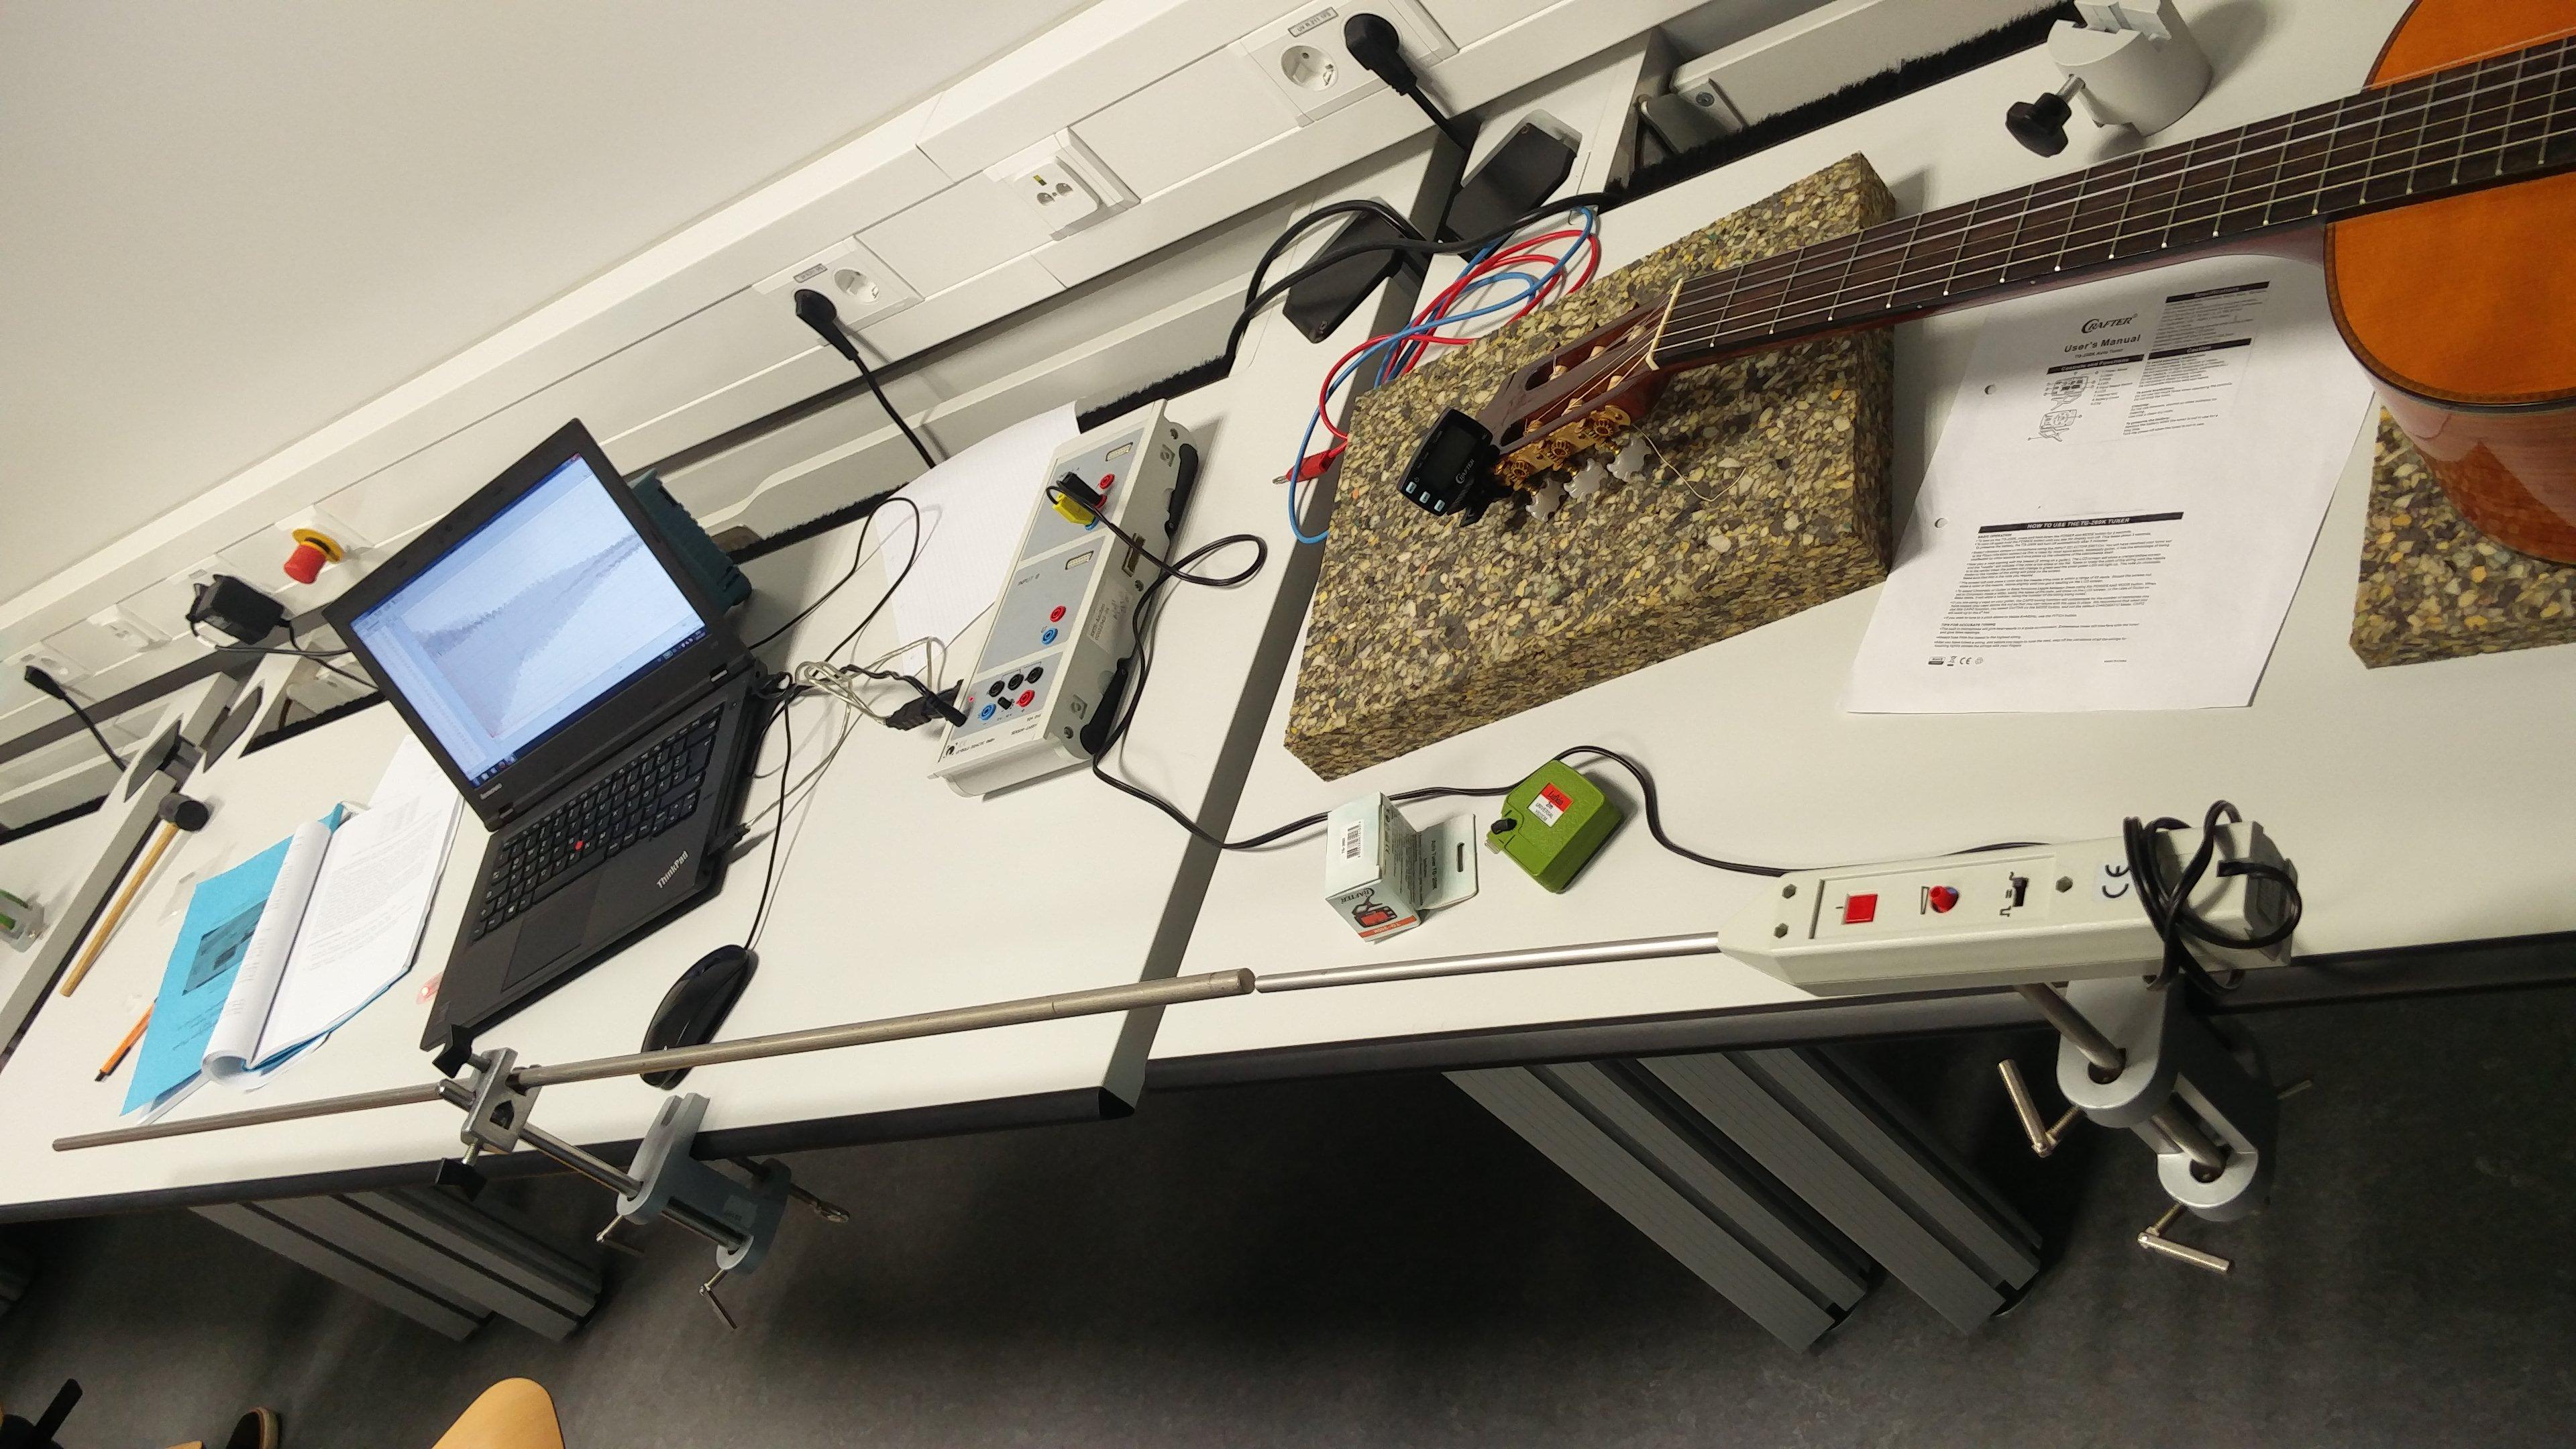
\includegraphics[scale=0.1]{../Stange.jpg}
	\caption{Aufbau zur Bestimmung der Elastizitätsodule}
	\label{fig:Aufbau zur Bestimmung der E-Module}
\end{figure}

\subsection{Auswertung}
Man bestimmt zuerst die Länge, die Dicke und die Masse der zu analysierenden Stäbe. Dazu misst man die Länge mithilfe eines Maßbandes, die Dicke mithilfe einer Mikrometerschraube und die Masse mithilfe einer Waage. Die Werte mit ihren Fehlern für die vier Metalle im Versuch sind in Tabelle \ref{table:Metalldaten} dargestellt. 

\begin{table}[H]
\centering
\renewcommand{\arraystretch}{1.2}
\begin{tabular}{|c|c|c|c|}
\hline Metall & Länge(in cm) & Durchmesser(in mm) & Masse(in g) \\
\hline Messing & $130 \pm 0,1$ &  $11,974 \pm 0,003$ & $1273,3 \pm 0,1$ \\
Eisen & $130,3 \pm 0,1$ &  $11.967 \pm 0,002$ & $1156,9 \pm 0,1$ \\
Kupfer & $129,9 \pm 0,1$ & $11.961 \pm 0,001$ & $1301,6 \pm 0,1$ \\
Aluminium & $129,9 \pm 0,1$ & $12.061 \pm 0,003$ & $399,04 \pm 0,1$ \\
\hline  
\end{tabular}
\caption{Gemessene Daten der vier Metalle}
\label{table:Metalldaten}
\end{table}

\noindent Dabei stammt der Fehler jeweils aus der Skala des verwendeten Messgeräts. Bei dem Durchmesser wurde über 6 Messungen gemittelt und der Fehler auf den Mittelwert bestimmt.
\\ Mithilfe einer FFT im \texttt{CASSY-Lab} lassen sich die Frequenzen bestimmen, mit der sich der Schall in der Stange bewegt. Dazu bestimmt man den Schwerpunkt der Peaks im Frequenzspektrum mit Hilfe der \texttt{CASSY-Lab}-Funktion(Abbildung \ref{FFt von Aluminium} und \ref{FFT von Eisen}). 
\begin{figure}[H]
	\begin{minipage}[t]{0.45\linewidth}
	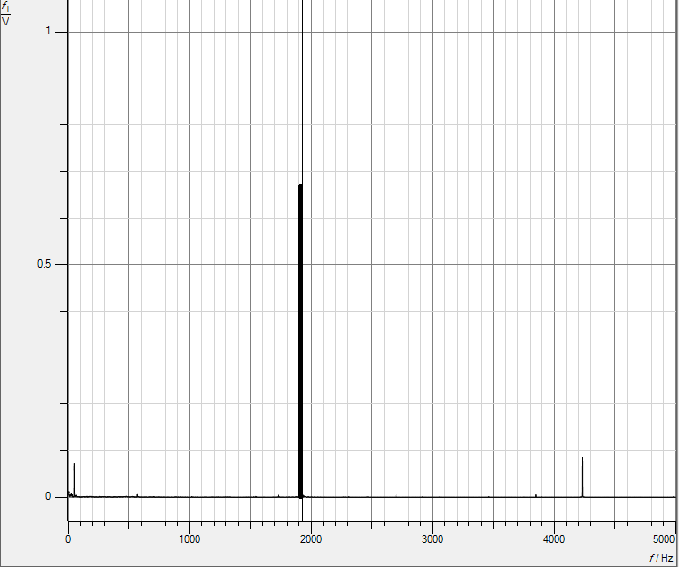
\includegraphics[scale=0.3]{../Aluminium.png}
	\caption{FFT von Aluminium}
	\label{FFt von Aluminium}
	\end{minipage}
	\hspace{0.1\linewidth}
	\begin{minipage}[t]{0.45\linewidth}
	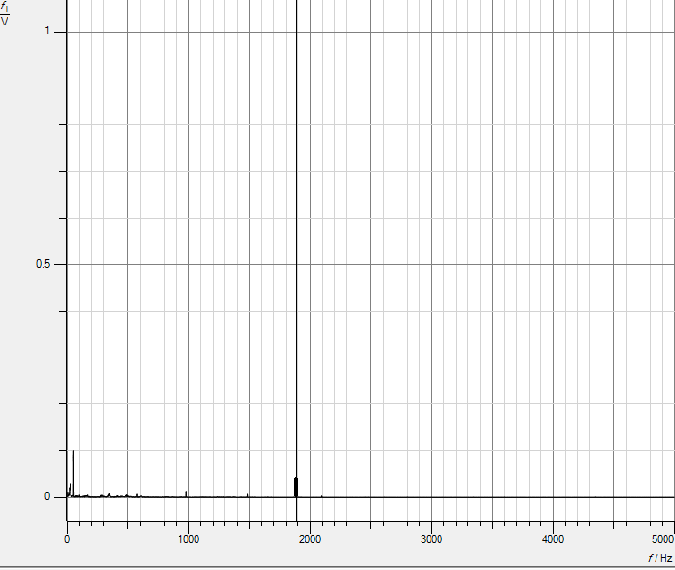
\includegraphics[scale=0.3]{../Eisen.png}
	\caption{FFT von Eisen}
	\label{FFT von Eisen}
	\end{minipage}
	\label{fig:Aufbau des Versuchs}
\end{figure}

\noindent Daraus ergibt sich die in \ref{fig:Peaks} zu sehende Peakverteilung bei 10-facher Messung der Schwingung in einem Metall.
Mithilfe einer FFT im \texttt{CASSY-Lab} lassen sich die Frequenzen bestimmen, mit der sich der Schall in der Stange bewegt. Dazu bestimmt man den Schwerpunkt der Peaks im Frequenzspektrum mit Hilfe der \texttt{CASSY-Lab}-Funktion. Daraus ergab sich die in \ref{fig:Peaks} zu sehende Peakverteilung bei 10-facher Messung der Schwingung in einem Metall.

\begin{figure}[H]
	\centering
	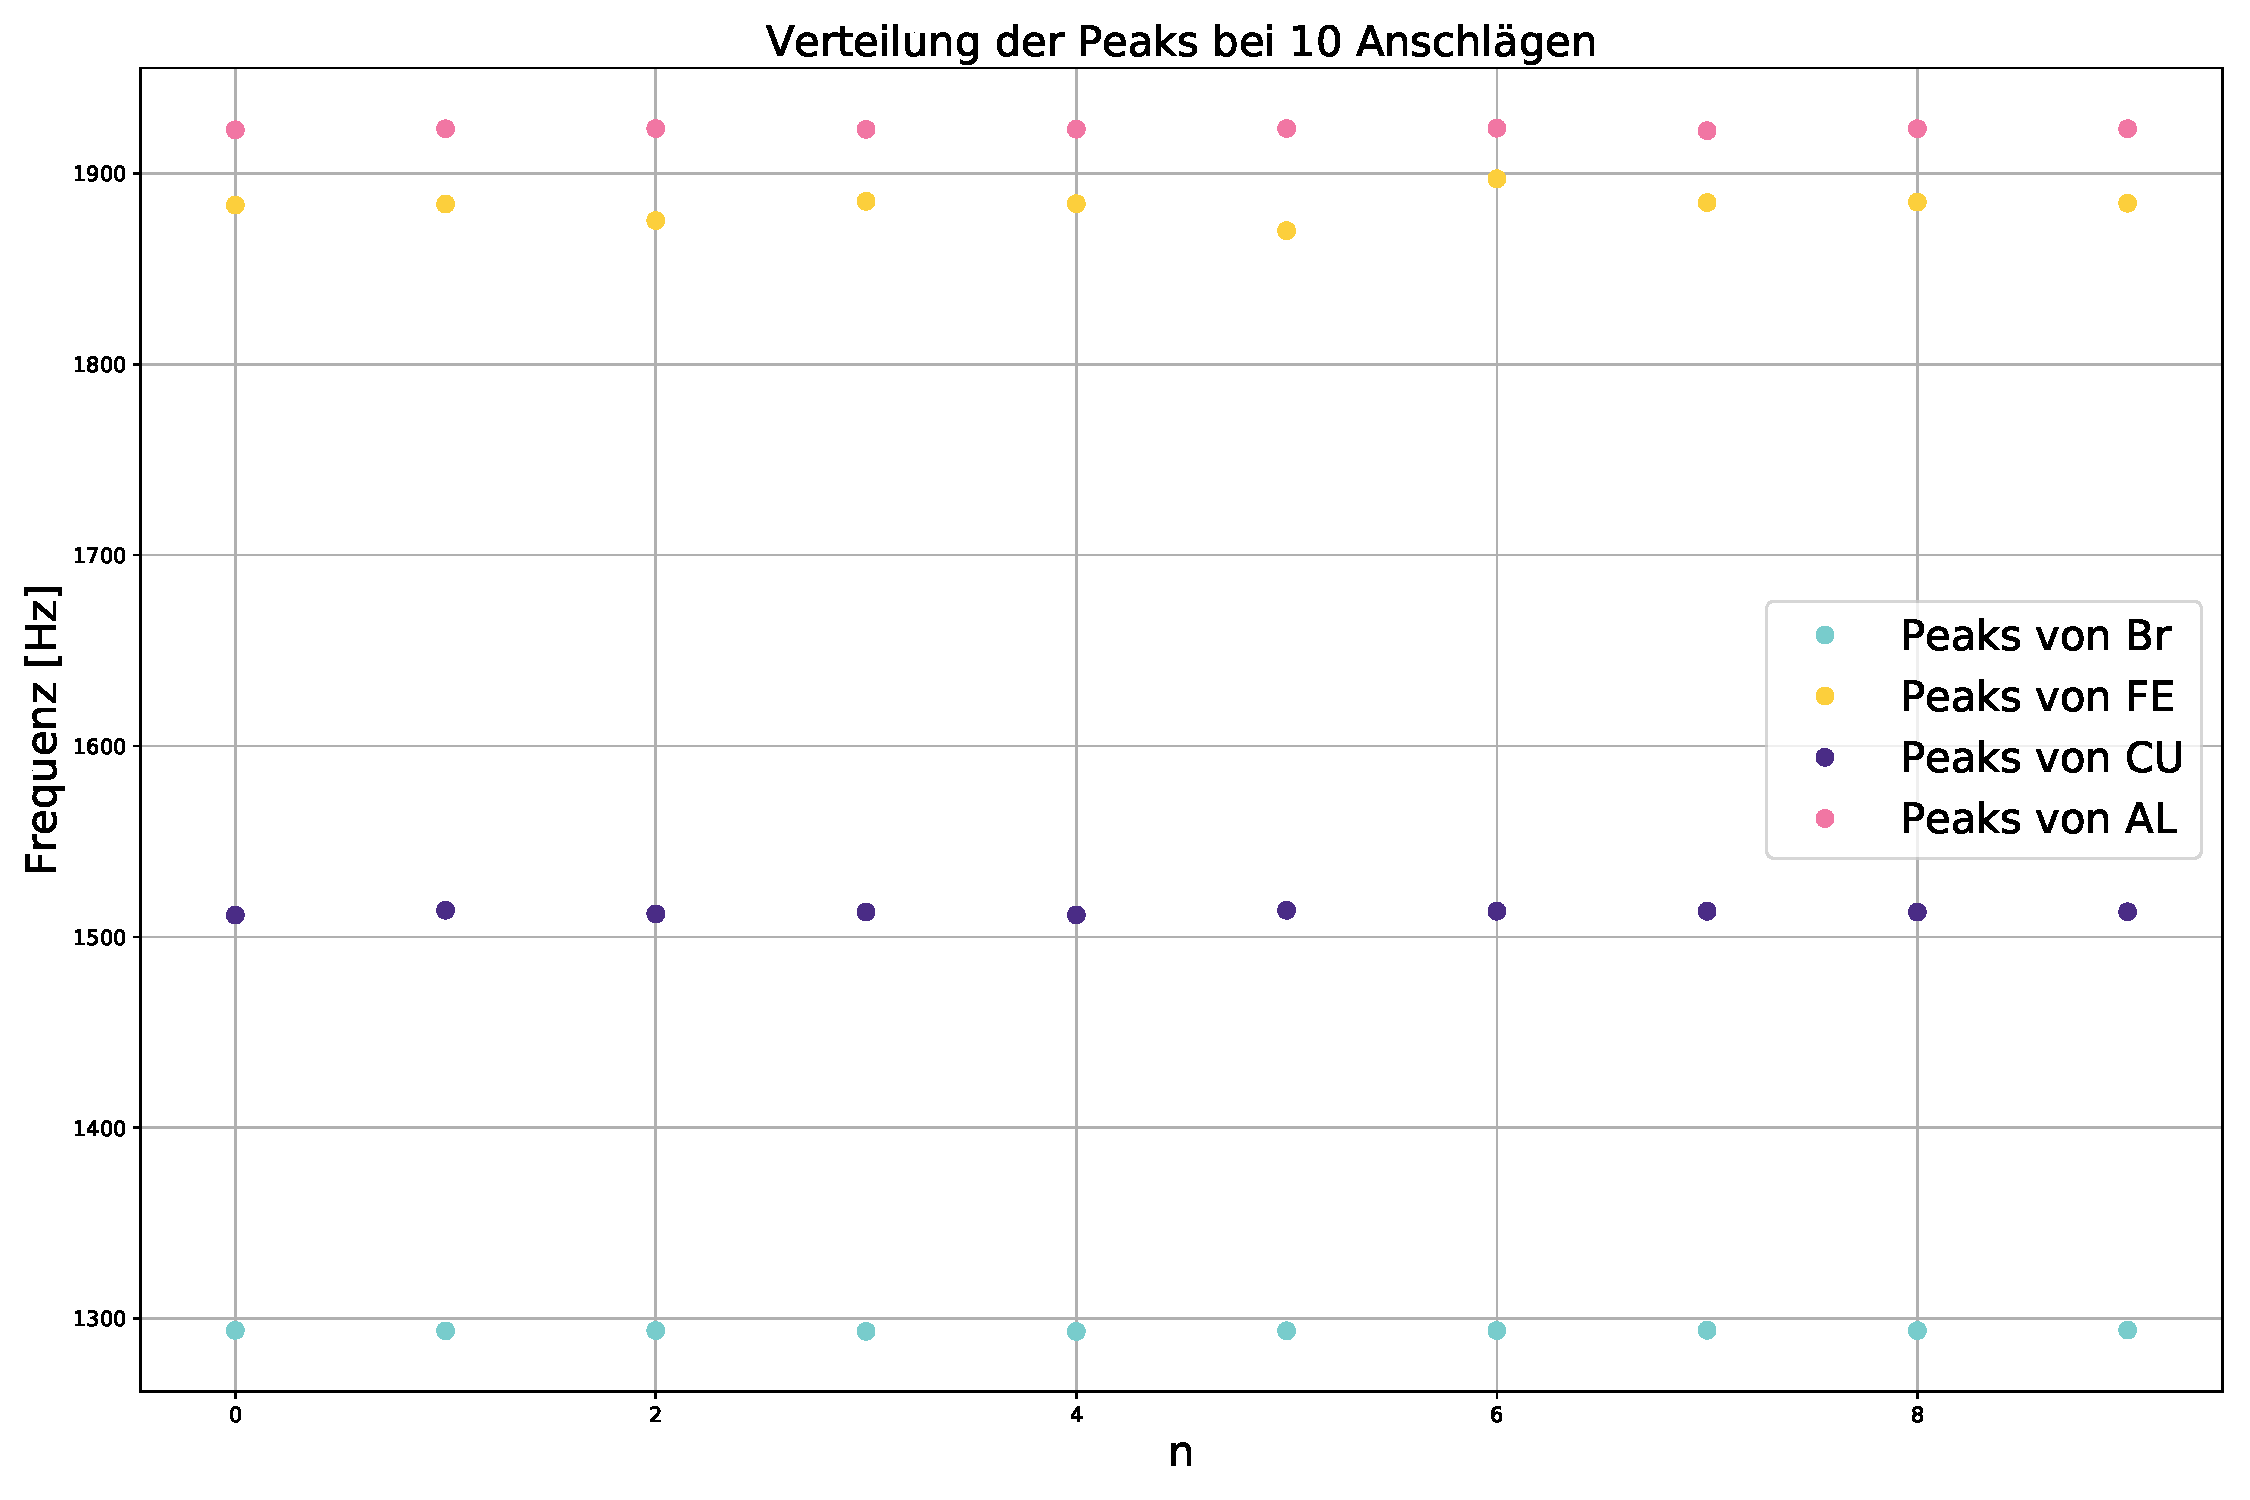
\includegraphics[scale=0.3]{../Plots/Peakverteilung.pdf}
	\caption{Schwingungen der E-Seite in den Bünden 0-9}
	\label{fig:Peaks}
\end{figure}

\noindent Bei einigen Messungen überwogen die Störfrequenzen in der FFT, wie am Beispiel von Eisen in der Abbildung \ref{FFT von Eisen} zu erkennen. Durch Bildung des Mittelwerts mit entsprechendem Fehler ergeben sich die in Tabelle \ref{table:Peaks} zu sehenden Frequenzen der Metalle. Es ist auffällig, dass bei Eisen die größten Schwankungen in der Schwingungsfrequenz gemessen werden.
Durch Bildung des Mittelwerts mit entsprechendem Fehler ergeben sich die in Tabelle \ref{table:Peaks} zu sehenden Frequenzen der Metalle.

\begin{table}[H]
\centering
\renewcommand{\arraystretch}{1.2}
\begin{tabular}{|c|c|c|}
\hline Metall & Frequenz(in Hz) & Geschwindigkeit(in $\frac{m}{s}$) \\
\hline Messing & $1293,63 \pm 0,07$ & $3363,438 \pm 2,594$ \\
Eisen & $1883,38 \pm 2,11$ & $4908,088 \pm 6,665$ \\
Kupfer & $1512,86 \pm 0,28$ & $3930,410 \pm 3,112$ \\
Aluminium & $1923,28 \pm 0,12$ & $4996,681 \pm 3,036$ \\
\hline
\end{tabular}
\caption{Gemessene Frequenzen der longitudinalen Schallwellen in den vier Metallen}
\label{table:Peaks}
\end{table}

\noindent Mit Hilfe der Formel \ref{eq:Emodul} kann man nun, mit den ermittelten Daten, die Elastizitätsmodule der Metalle bestimmen. Der Fehler auf das Elastizitätsmodul ergibt sich aus dem Gaußschen Fehlerfortpflanzungsgesetz:
\begin{equation}
\sigma_E = E \cdot \sqrt{\left(\frac{\sigma_L}{L}\right)^2 + \left(\frac{\sigma_M}{M}\right)^2 + 4 \cdot \left(\frac{\sigma_D}{D}\right)^2 + 4 \cdot \left(\frac{\sigma_f}{f}\right)^2}.
\end{equation} 
wobei die Fehler der Frequenz und des Durchmessers am stärksten einfließen.
Daraus ergeben sich die Elastizitätsmodule für die vier Metalle, die in der Tabelle \ref{Tabelle 3} abgebildet sind.  

\begin{table}[H]
\centering
\large
\renewcommand{\arraystretch}{1.2}
\begin{tabular}{|c|c|}
\hline Metall & Elastizitätsmodul (in $10^{10} \frac{N}{m^2}$) \\
\hline Messing & $9,5616 \pm 0,0732$ \\
Eisen & $19,0000 \pm 0,0455$ \\
Kupfer & $13,7760 \pm 0,0120$ \\
Aluminium & $6,7130 \pm 0,0643$ \\
\hline
\end{tabular}
\caption{Elastizitätsmodule}
\label{Tabelle 3}
\end{table}

Es fällt auf, dass Eisen das höchste und Aluminium das geringste Elastizitätsmodul hat.

\subsection{Fazit}
Verglichen mit den Literaturwerten, sind die ermittelten Elastizitätsmodule im Bereich der angegebenen Intervalle. Ein großes Problem dabei war es die Stange in einer Ebene anzuschlagen. Dies führte dazu, dass die Stangen in alle Richtungen schwingen konnten, nicht wie gewünscht. Außerdem nahm das Mikrofon auch jegliche Art von Hintergrundgeräuschen wie etwa Gespräche auf. Im Frequenzspektrum waren daher noch andere Peaks zu sehen, die im schlimmsten Fall, viel höher als die der Grundschwingung waren. 
Ein weiteres Problem bestand darin, dass mit den anderen, im Raum befindlichen Gruppen, so zu koordinieren, dass immer nur eine Gruppe dieselbe Stange anschlägt.

\newpage
\section{Physik der Gittare}
\subsection{Grundlagen}
Schlägt man eine Saite an, breiten sich die Schwingungen in Form von Transversalwellen in beide Richtungen aus. Am Steg und am Sattel werden die Transversalwellen reflektiert, wodurch stehende Wellen entstehen. Dabei muss am festen Ende ein Phasensprung von $\Delta \phi = \pi$ auftreten. Die Knoten liegen dabei an den Saitenenden. Mit der folgenden Beziehung kann man die Auslenkung einer Saite bei stehenden Welle beschreiben
\begin{equation}
y(x,t) = \sum_{n=1}^{\infty} A_n\cos(\omega_nt+\phi_n)\sin(k_nx).
\end{equation}

Beim gleichzeitigen Anschlagen von zwei Saiten mit leicht verschiedenen Frequenzen entsteht eine Schwebung mit den Frequenzen
\begin{equation}
\omega_{sch} = \frac{\omega_2 - \omega_1}{2} \qquad \omega_{res} = \frac{\omega_2 + \omega_1}{2}
\end{equation}

Außer der Grundschwingung entstehen Oberschwingungen mit der Wellenlänge
\begin{equation}
\lambda_n = \frac{2L}{n} \quad mit \quad  n = 1,2,... .
\end{equation}

Die Schwingung einer Saite ist außerdem Abhängig von ihrem Material, wobei [T] = N die Saitenspannung und $[\mu] = \frac{kg}{m}$ den Massebelag beschreiben. Die Herstellerangaben für die im Versuch ausgemessenen Saiten finden sich in Tabelle \ref{table:Saitenmaterial}.

Wenn die Saite in verschiedenen Bünden mit den Längen $L_n$ angeschlagen wird gilt für die Frequenzen der Grundschwingung die Beziehung \ref{eq:fn}
\begin{equation}\label{eq:fn}
f_n = \frac{1}{2 L_n} \cdot \sqrt{\frac{T}{\mu}},
\end{equation} 


Bei einer Bewegung wie in Abbildung \ref{fig:Bewegungsverlauf einer Saite, angeschlagen in der Mitte} treten nur die Schwingungsmoden auf, die bei denen im Zentrum Schwingungsbäuche auftreten(alle ungeraden Harmonischen. Das Frequenzspektrum enthält daher nur alle ungeraden Vielfachen der Grundfrequenz und ist somit abhängig vom Anschlagspunkt.
\begin{figure}[H]
	\centering
	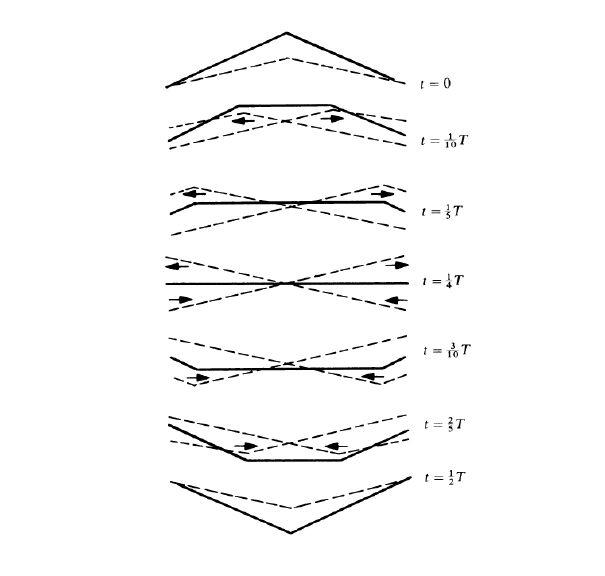
\includegraphics[scale=0.4]{../Bewegungsverlauf.jpg}
	\caption{Bewegungsverlauf einer Saite, angeschlagen in der Mitte}
	\label{fig:Bewegungsverlauf einer Saite, angeschlagen in der Mitte}
\end{figure}

\subsection{Aufbau und Durchführung}
Die Gitarre liegt auf einer dicken Polsterung und das Mikrofon, dass mit einem Cassy-Modul verbunden ist, wird oberhalb des Stimmloches in einem Abstand von ca 15 cm aufgestellt. 
Mit einem Stimmgerät wird die Gitarre vor einer Messung gestimmt. Das Mikrofon ist ein Schalldruckempfänger(von Leybold Didactic GmbH). Dieser wird dann mit dem Sensor-Cassy verbunden und wird im Amplitudenmodus mit einer Empfindlichkeit, die zu einer sinnvollen Datenaufzeichnung führt, eingestellt.
\begin{figure}[H]
	\centering
	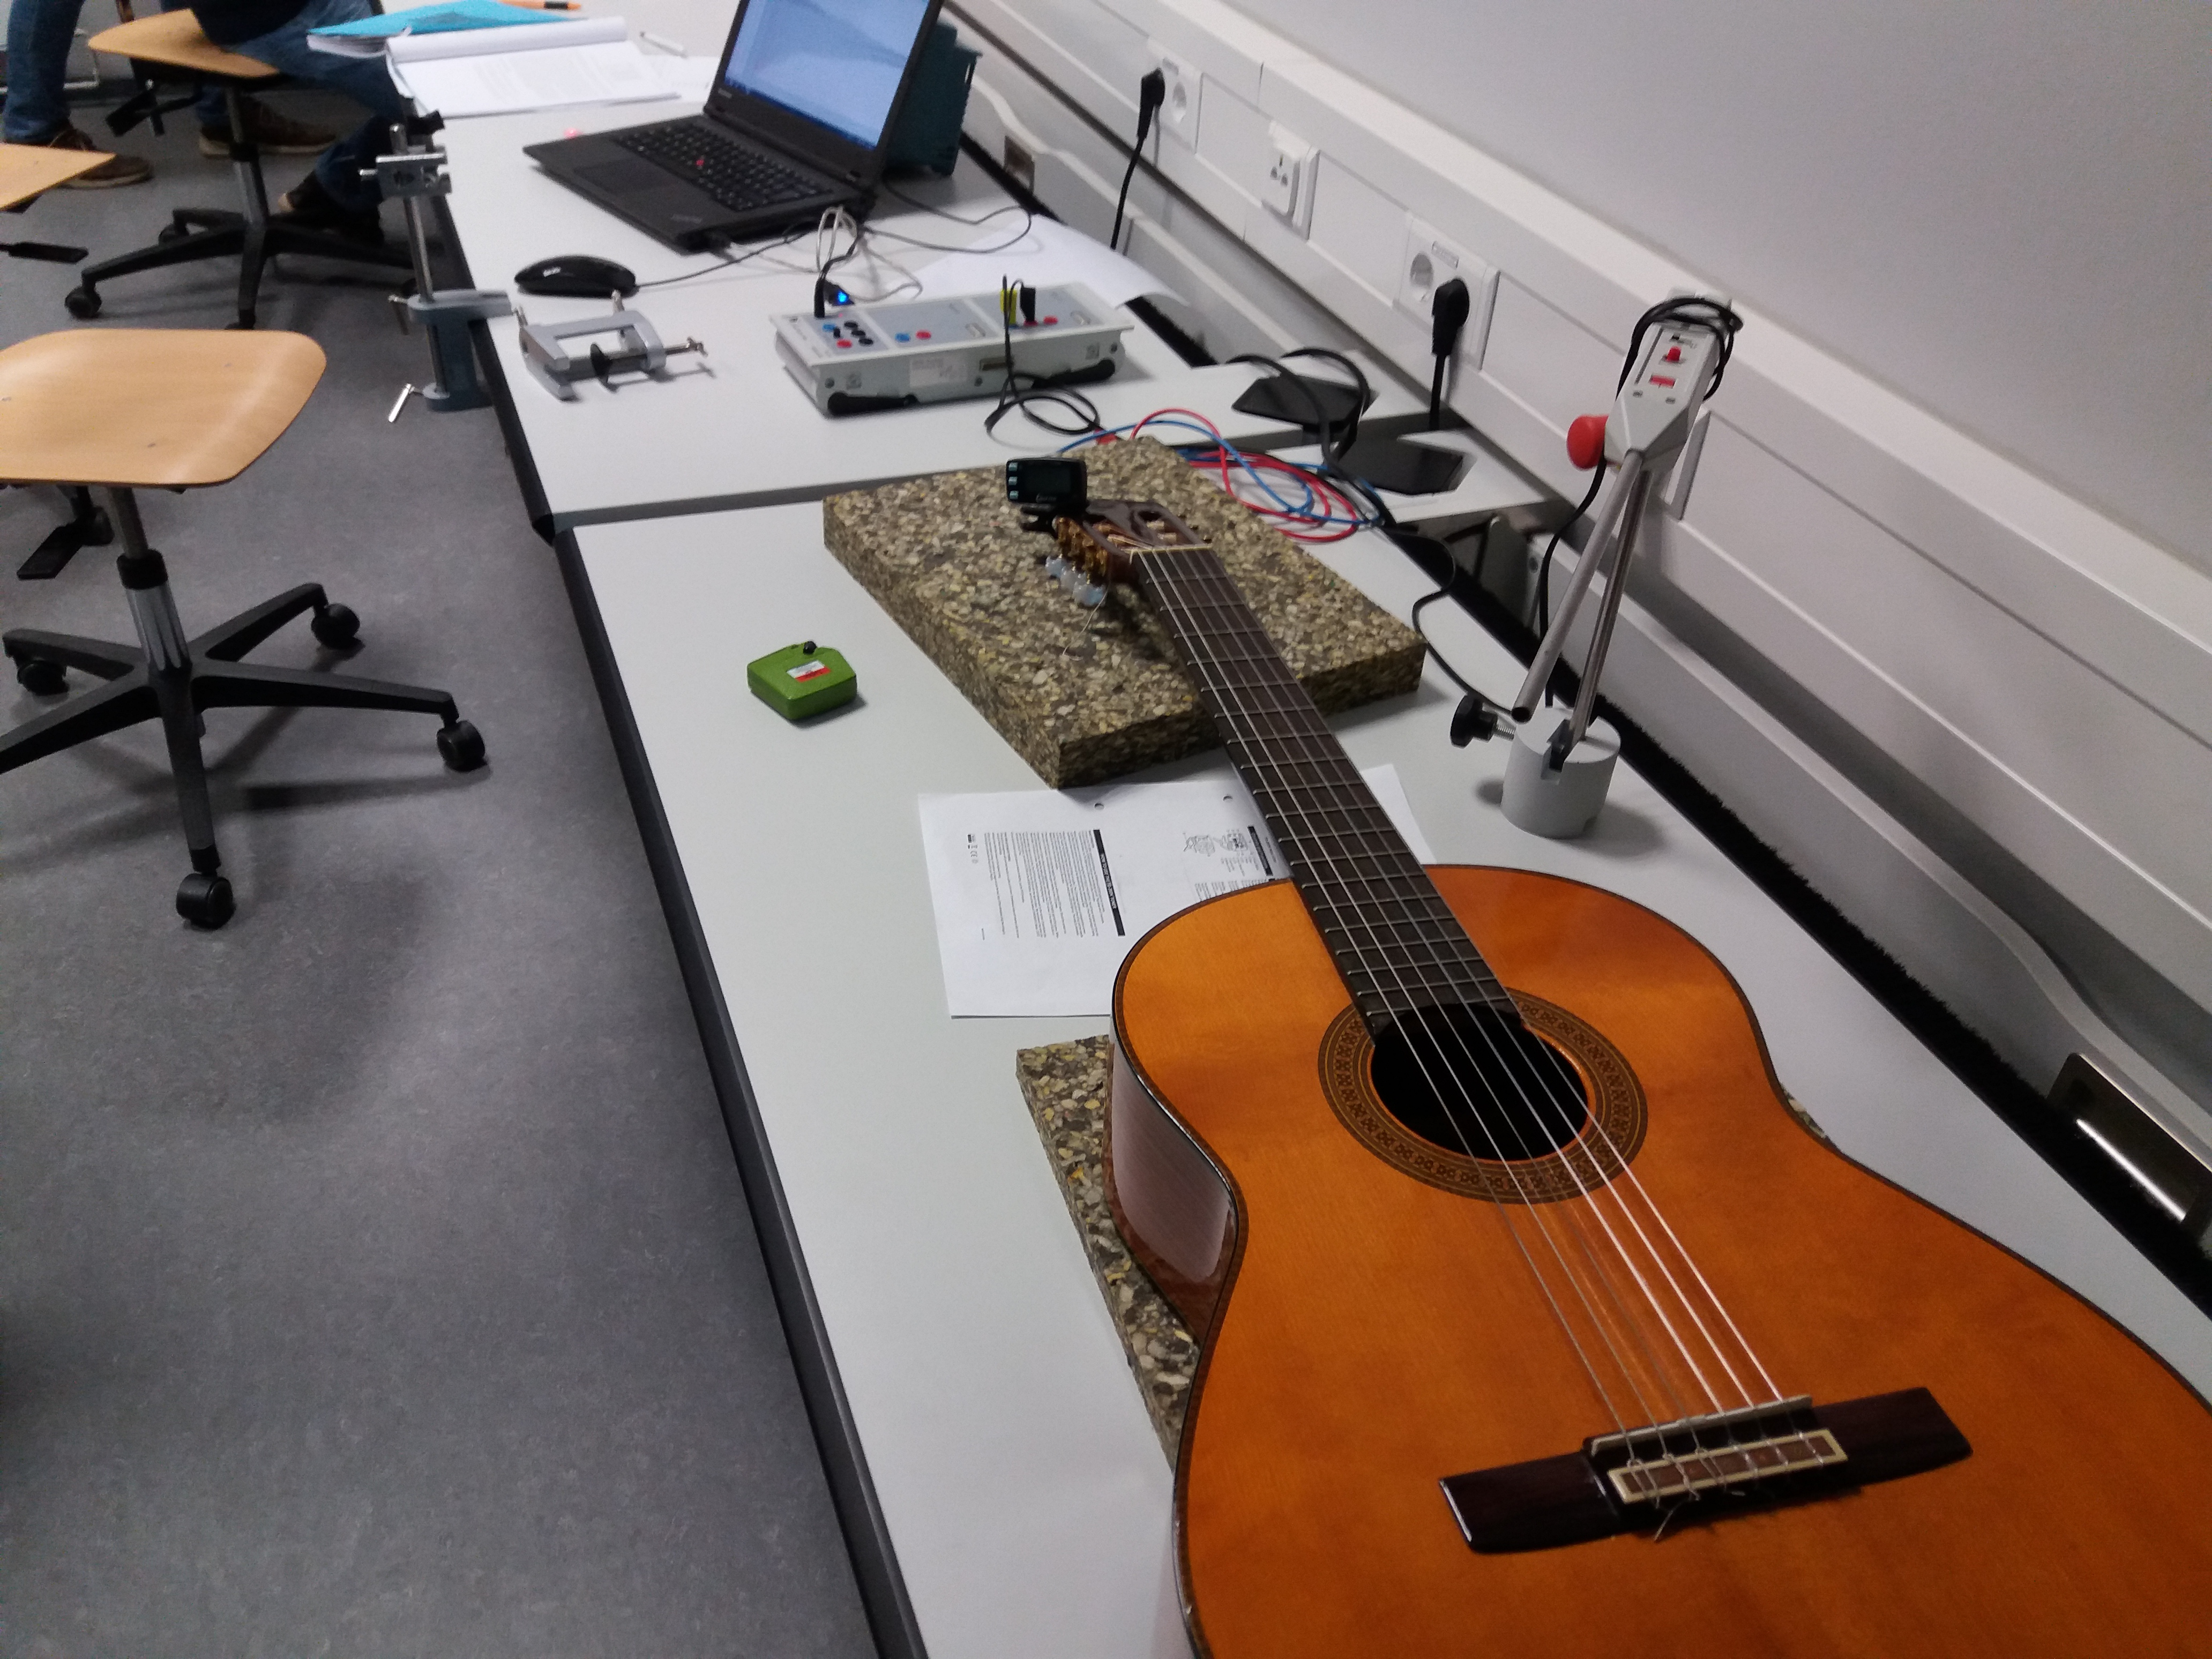
\includegraphics[scale=0.05]{../Gitarre.jpg}
	\caption{Aufbau des Versuchs}
	\label{fig:Aufbau des Versuchs}
\end{figure}

\subsubsection{Messung der Schwebung}
Mithilfe eines Stimmgerätes, wird eine Saite durch drehen der Stimmmechanik leicht verstimmt. Im Anschluss werden beide Saiten angeschlagen. Anhand des Spannungsbildes und des Frequenzspektrums, das mit dem Cassy-Modul aufgenommen wird, kann man nun die Schwebungsfrequenz $\omega_{sch}$ und die resultierende Frequenz $\omega_{res}$ bestimmen. Wird eine Saite zu stark verstimmt, lässt sich keine Schwebung erzeugen. Die beiden Saiten müssen möglichst gleichzeitig angeschlagen werden.

\subsubsection{Bestimmung der Saitenspannung}
Zur Bestimmung der Saitenspannung werden zunächst die Längen der Saiten ausgemessen. Im Anschluss werden die Frequenzen zweier beliebigen Saiten aufgenommen, abhängig vom abgeklemmten Bund, angefangen bei der leeren Saite. Für eine erfolgreiche Datenaufzeichnung muss die Abtastrate und die Anzahl der Messpunkte im Cassy geeignet gewählt werden. Es werden 10 verschiedene Messungen durchgeführt.  
Durch Auftragung der Frequenzen über die gemessenen Längen, abhängig vom Bund, entsteht ein linearer Zusammenhang, sodass $T/\mu$ abgelesen werden kann.  

\subsubsection{Aufnahme eines Frequenzspektrums} 
Eine bestimmte Saite wird zuerst bei der Hälfte, also im 12. Bund senkrecht angeschlagen. Die Schwingung wird auch hier mit einem Cassy-Modul aufgezeichnet und dann damit das Frequenzspektrum bestimmt. Anschließend wird die Saite bei einem anderen Abständen angeschlagen, z.B. bei $1/10, 1/5 \dots$ ihrer Länge.

\subsection{Auswertung}
\subsubsection{Schwebung}
Wie in der Durchführung schon beschrieben, wird eine Saite leicht verstimmt, sodass eine Schwebung erzeugt werden kann. Es werden die Saiten A und D genommen, wobei die Saite D leicht verstimmt und die Saite A im fünften Bund abgegriffen wird. Die Schwebungsfrequenz wird einmal aus den Eigenfrequenzen der schwingenden Saiten aus der FFT bestimmt und mit der Gleichung für $\omega_{sch}$ berechnet und mit der aus dem Spannungsverlauf abgelesenen Frequenz verglichen. Dazu wird die Zeitspanne durch die Anzahl der vollen Perioden geteilt. Der Kehrwert der so bestimmten Periode bildet die Schwebungsfrequenz. In den Abbildungen \ref{Abbildung 5} und \ref{Abbildung 6} sind diese abgebildet. Dazu werden zwei Messungen durchgeführt. Bei den Messungen wird der Schwerpunkt der beiden  Eigenfrequenzen  bestimmt. 
\begin{figure}[H]
	\begin{minipage}[t]{0.45\linewidth}
	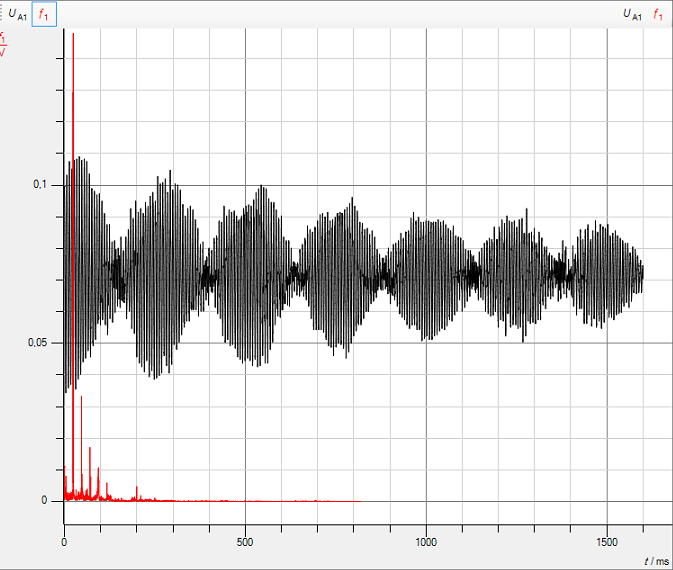
\includegraphics[scale=0.4]{../Schwebung1.png}
	\caption{Spannungsverlauf der Schwebung aus der ersten Messung}
	\label{Abbildung 5}
	\end{minipage}
	\hspace{0.1\linewidth}
	\begin{minipage}[t]{0.45\linewidth}
	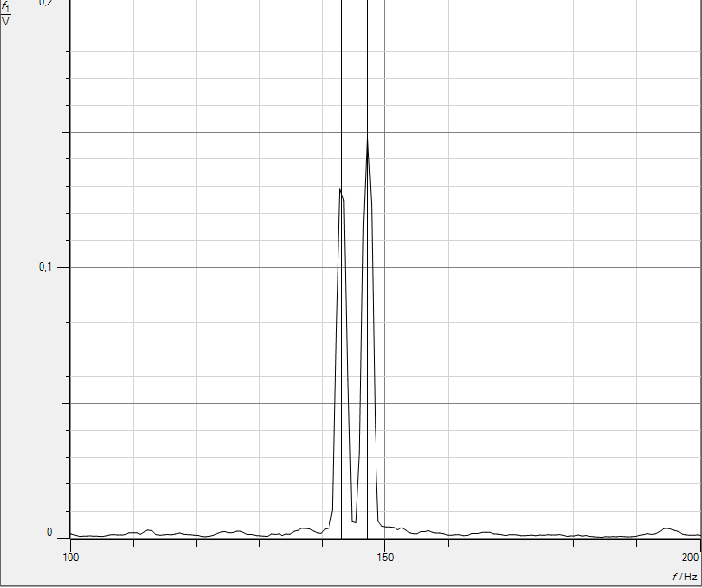
\includegraphics[scale=0.4]{../Schwebung1F.png}
	\caption{FFT der Schwebung aus der ersten Messung mit dem Peak-Schwerpunkt}
	\label{Abbildung 6}
	\end{minipage}
	\label{fig:Aufbau des Versuchs}
\end{figure}
\begin{figure}[H]
	\begin{minipage}[t]{0.45\linewidth}
	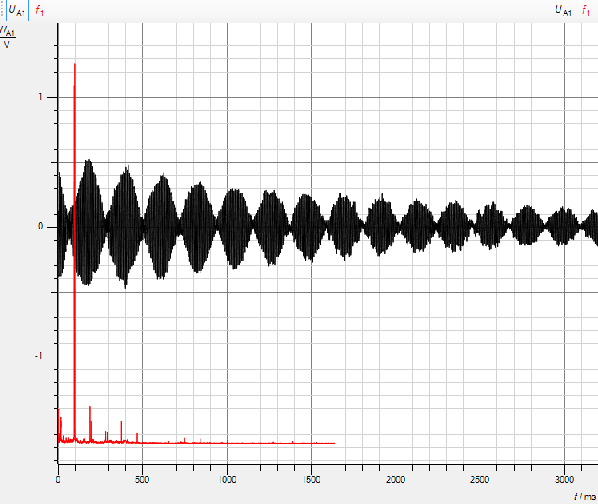
\includegraphics[scale=0.4]{../Schwebung2.png}
	\caption{Spannungsverlauf der Schwebung aus der zweiten Messung}
	\label{Abbildung 5}
	\end{minipage}
	\hspace{0.1\linewidth}
	\begin{minipage}[t]{0.45\linewidth}
	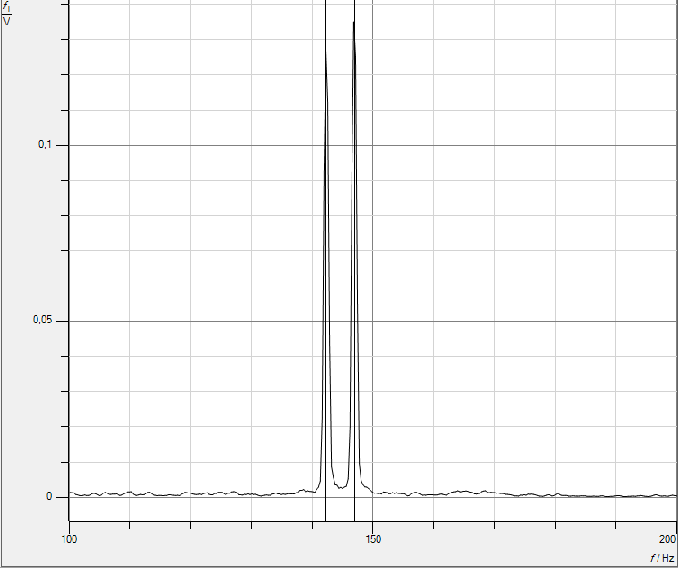
\includegraphics[scale=0.4]{../Schwebung2F.png}
	\caption{FFT der Schwebung aus der zweiten Messung mit dem Peak-Schwerpunkt}
	\label{Abbildung 6}
	\end{minipage}
	\label{fig:Aufbau des Versuchs}
\end{figure}

Der Fehler auf die Periode ist durch 
\begin{equation}
\sigma_T = \frac{\surd2 \cdot \sigma_t}{n}
\end{equation}
gegeben, der Fehler auf dem Peak ist der Kehrwert der gemessenen Zeitspanne und der Fehler auf die Schwebungsfrequenz wird über
\begin{equation}
\sigma_{f_{sch}} = \frac{\sigma_T}{T^2}. 
\end{equation}
bestimmt. Die Ergebnisse der Messungen sind in der Tabelle \ref{Tabelle 4} zu finden.
\begin{table}[H]
\centering
\renewcommand{\arraystretch}{1.2}
\begin{tabular}{|c|c|c|c|}
\hline Messung & $f_1,f_2$ aus FFT & $f_{sch}$ aus FFT & $f_{sch}$ abgelesen \\
\hline $1$ & $143,04 \pm 0,625 Hz$ & & \\
           & $147,14 \pm 0,625 Hz$ & $2,050 \pm 0,44 Hz$ & $2,064 	\pm 2,0 \cdot 10^{-4} Hz $ \\
\hline $2$ & $142,29 \pm 0,625 Hz$ &  &    \\
 		& $146,89 \pm 0,625 Hz$ & $2,300 \pm 0,44 Hz$  & $2,298 \pm 1,2 \cdot 10^{-4} Hz$ \\
\hline
\end{tabular}
\caption{Ergebnisse aus der zweiten Messung}
\label{Tabelle 4}
\end{table}


\subsubsection{Saitenspannung}
Bei diesem Versuch werden die Saiten A und E analysiert. Dazu werden jeweils zehn Frequenzen aufgenommen, die bei unterschiedlichen Bunden abgegriffen werden. Zuerst wird die Länge, abhängig vom Bund aus, gemessen. Die Längen sind in der Tabelle \ref{Saitenlängen bei verschiedenen Bunden} aufgelistet.
Die Angaben des Herstellers zu den Materialeigenschaften der verwendeten Saiten sind in Tabelle \ref{table:Saitenmaterial} zu sehen.

\begin{table}[H]
	\centering
	\renewcommand{\arraystretch}{1.2}
	\begin{tabular}{|c|c|c|}
		\hline
		Saite & $\mu \;[\frac{kg}{m}]$ & $T \;[N]$  \\
		\hline 
		A & $3.4095 \cdot 10^{-3}$ & $68.04$ \\
		E & $5.6712 \cdot 10^{-3}$ & $63.50$\\
		\hline
	\end{tabular}
	\caption{Herstellerangaben zum Saitenmaterial}
	\label{table:Saitenmaterial}
\end{table}

\begin{table}[H]
\centering
\renewcommand{\arraystretch}{1.2}
\begin{tabular}{|c|c|}
\hline Bund & Länge [cm] \\
\hline $1$ & $65,2 \pm 0,1$ \\
$2$ & $61,6 \pm 0,1$ \\
$3$ & $58,2 \pm 0,1$ \\
$4$ & $51,9 \pm 0,1$ \\
$5$ & $49,0 \pm 0,1$ \\
$6$ & $46,2 \pm 0,1$ \\
$7$ & $43,6 \pm 0,1$ \\
$8$ & $41,2 \pm 0,1$ \\
$9$ & $38,9 \pm 0,1$ \\
\hline
\end{tabular}
\caption{Saitenlängen bei verschiedenen Bunden}
\label{Saitenlängen bei verschiedenen Bunden}
\end{table}


Zur Bestimmung der Materialeigenschaften der Saite wurde eine Auftragung der Frequenz über $1/2L$ gewählt und eine lineare Regression durchgeführt. Bei dieser wurden sowohl die Fehler in y-Richtung (Peakfehler als Abstand von zwei Frequenzen in der FFT von $1/T_{ges} = 1/0.8s = 1.25 Hz$) als auch in x-Richtung (Skala des Maßbandes bei der Längenmessung: $1mm$) berücksichtigt. Dadurch dass im $\chi^2$ und Residuenplot der kombinierte Fehler $\sqrt{\sigma_y^2+f'(x)\sigma_x^2}$ einfließt und für die Gerade hier $f'(x)=a$ sehr groß ist, werden die Fehler auf die Messpunkte sehr groß und das $\chi^2/ndf$ entsprechend klein.
Beide Geraden gehen gut durch die Messpunkte durch, wodurch der Fehler auf die Fitparameter klein ausfällt.

\begin{figure}[H]
	\centering
	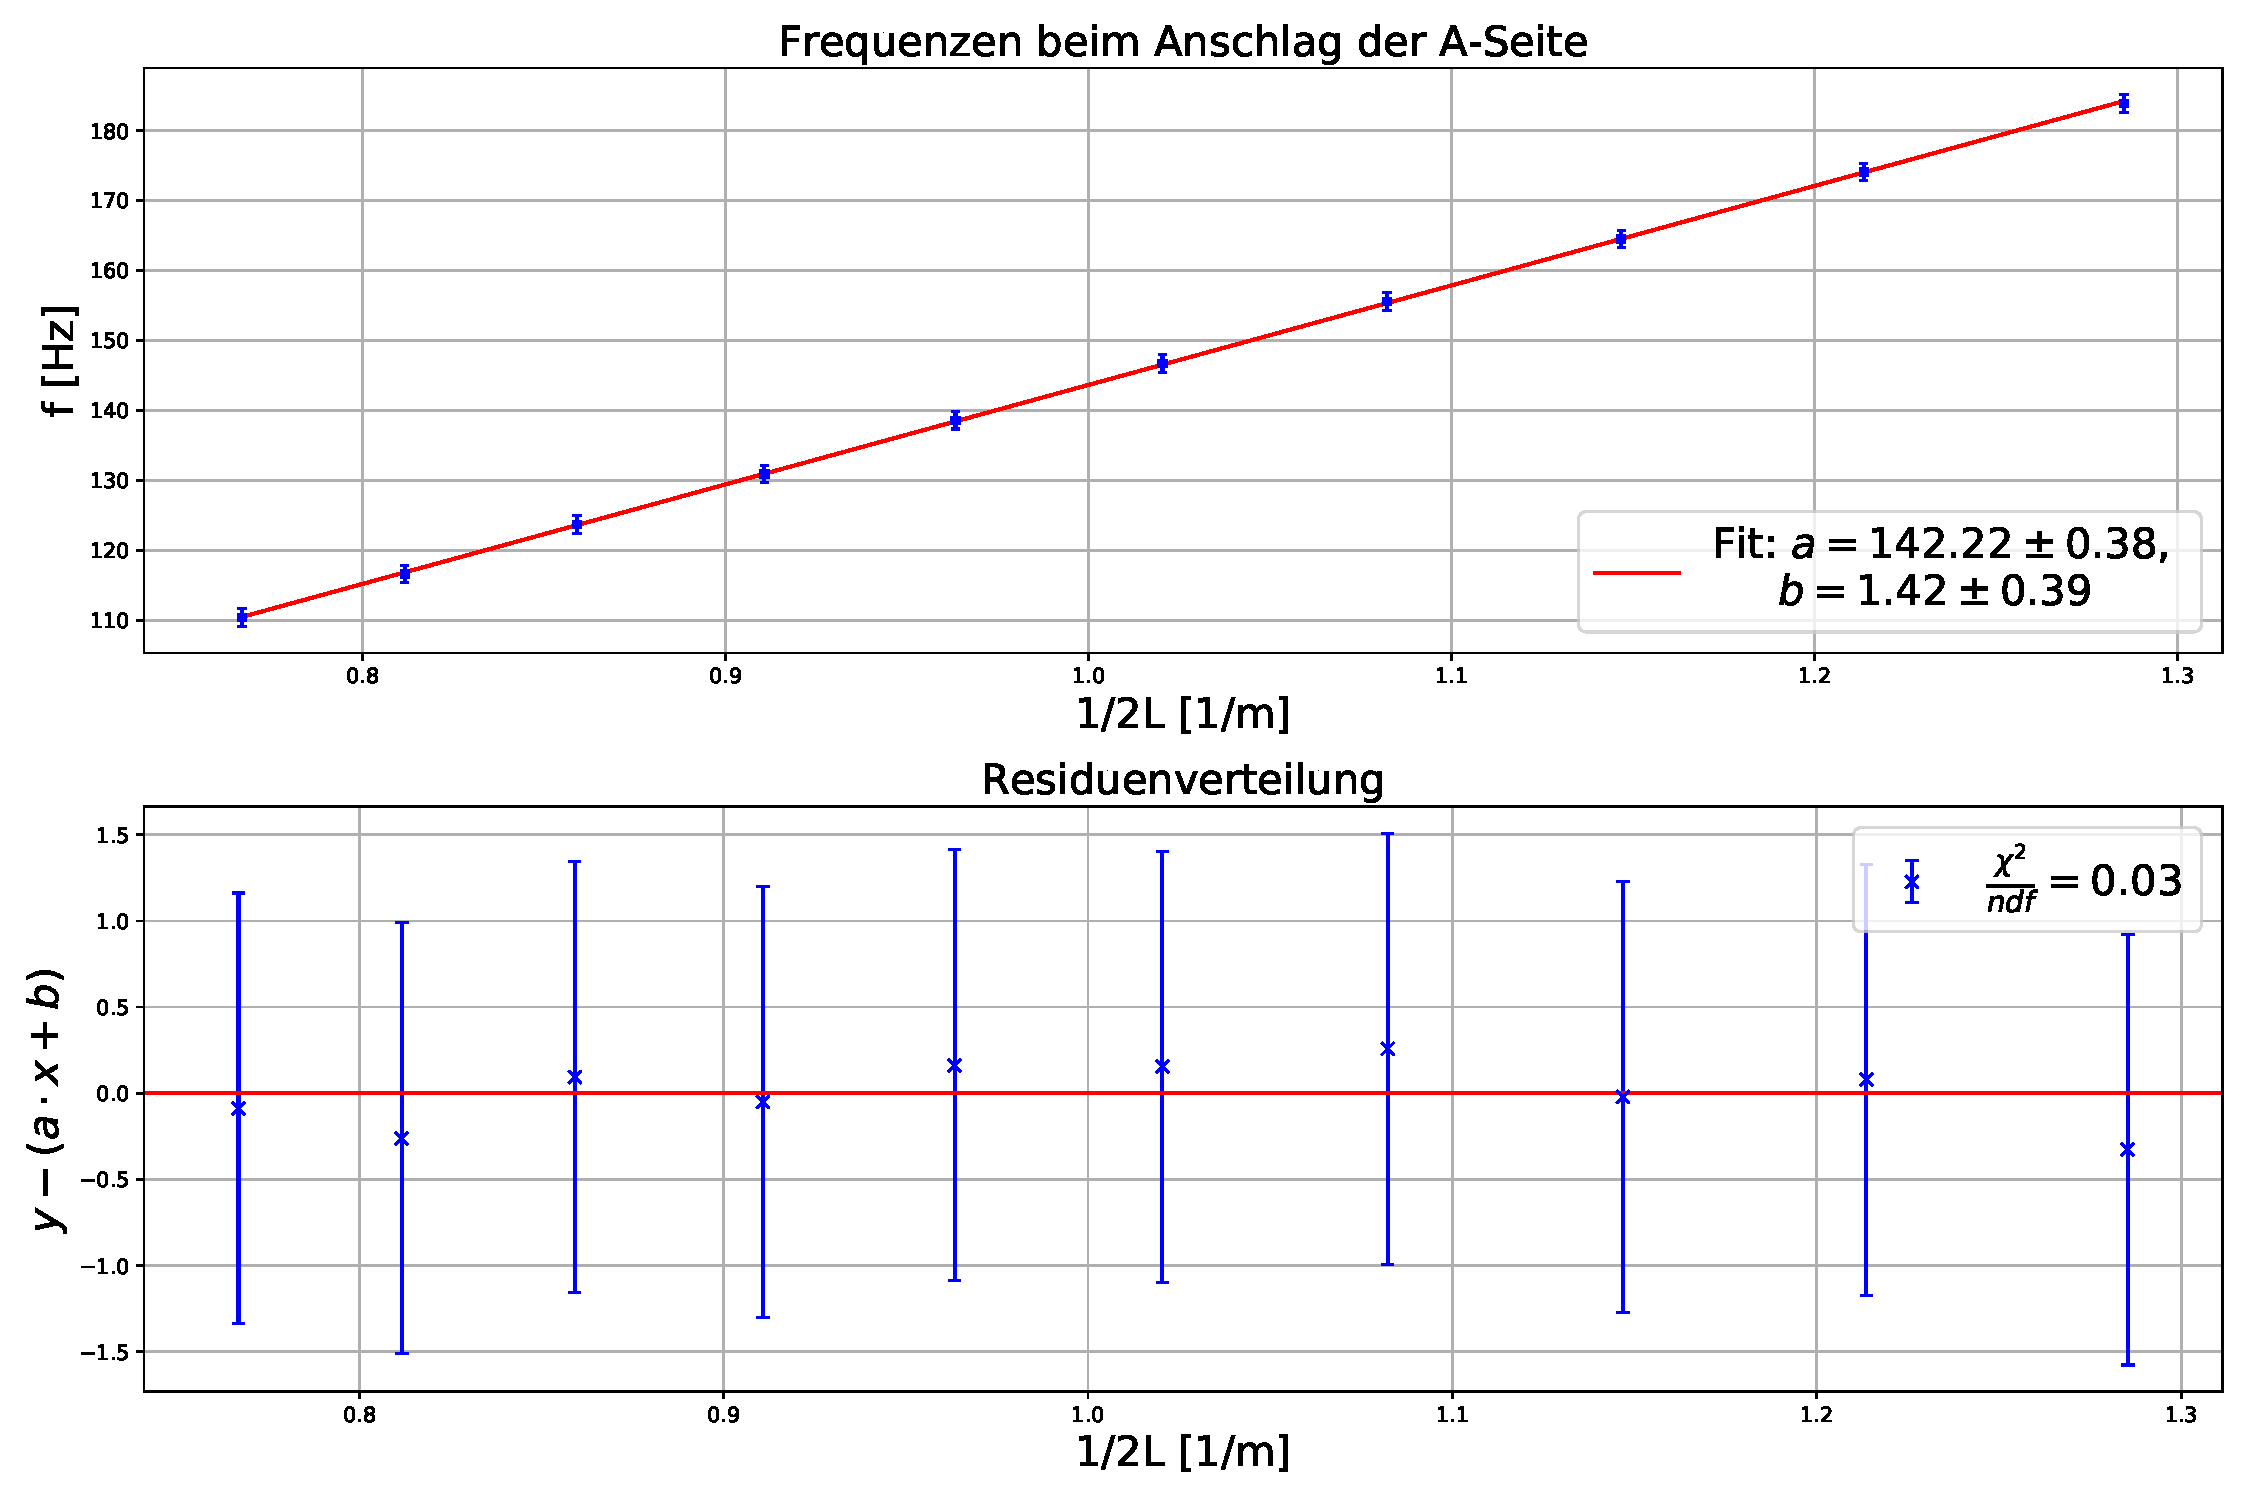
\includegraphics[scale=0.45]{../Plots/A-Seite.pdf}
	\caption{Schwingungen der A-Seite in den Bünden 0-9}
	\label{fig:ASaite}
\end{figure}
\begin{figure}[H]
	\centering
	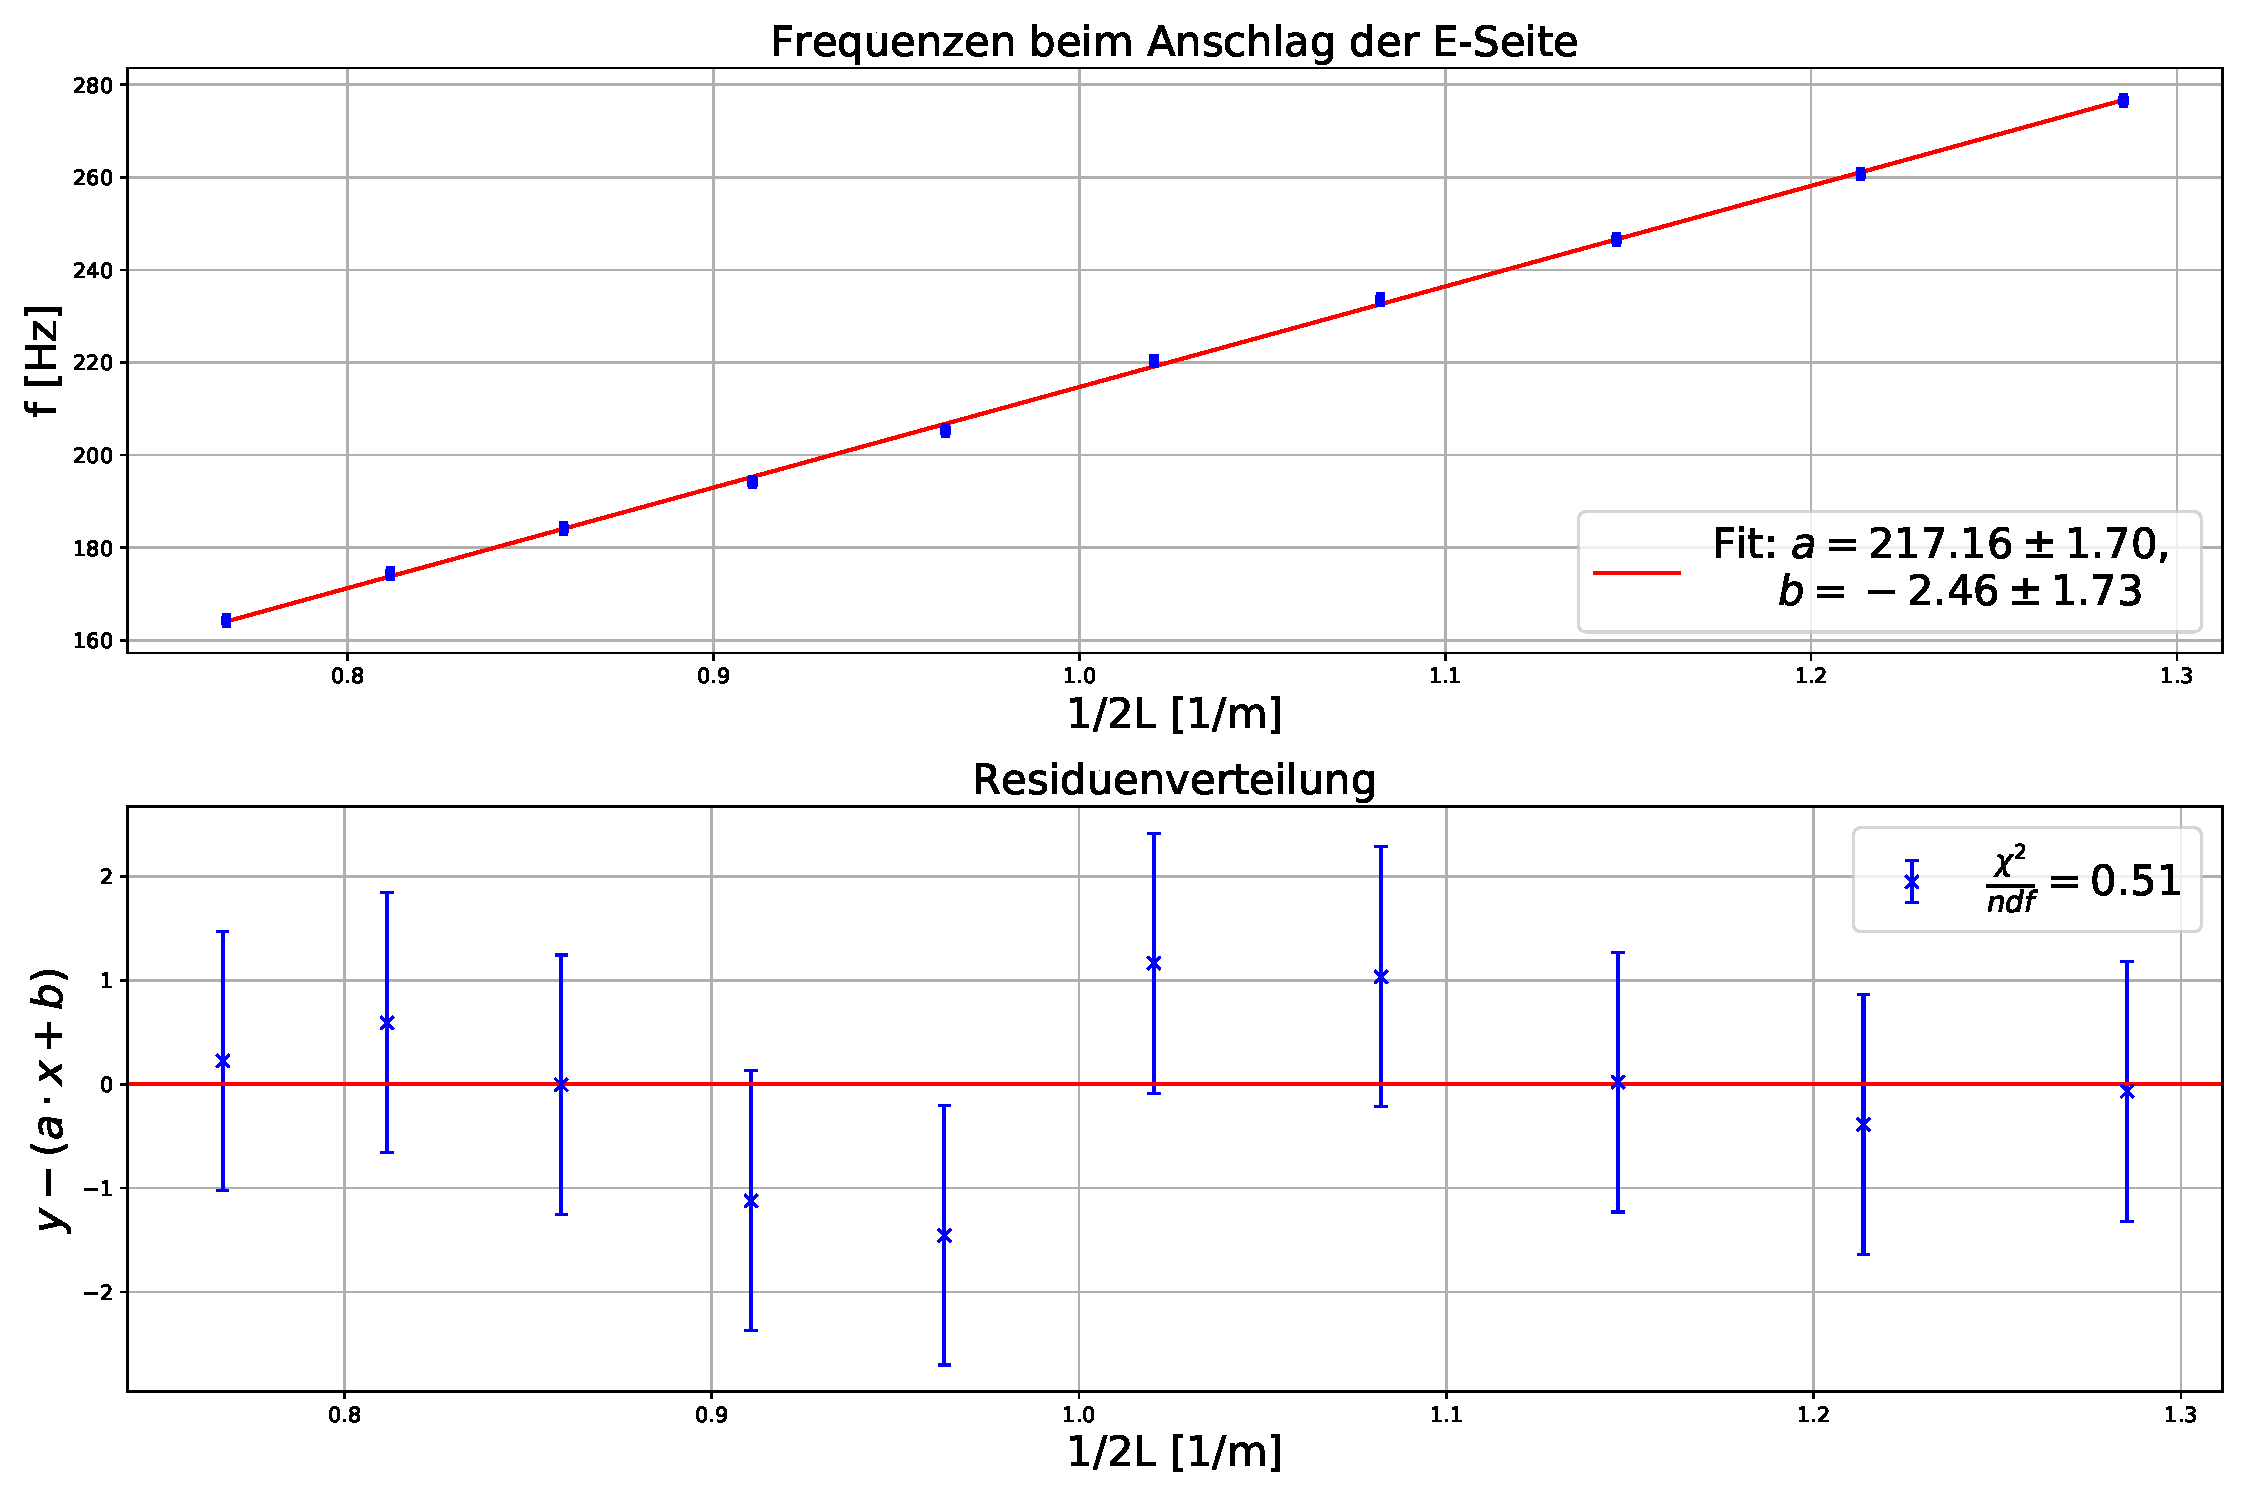
\includegraphics[scale=0.45]{../Plots/E-Seite.pdf}
	\caption{Schwingungen der E-Seite in den Bünden 0-9}
	\label{fig:ESaite}
\end{figure}

Das Verhältnis $\sqrt{T/\mu}$, was der Steigung $a$ der Geraden im Fit entspricht, lässt sich mit den  Herstellerangaben in Tabelle  \ref{table:Saitenmaterial} vergleichen.
 
\begin{table}[H]
	\centering
	\renewcommand{\arraystretch}{1.2}
	\begin{tabular}{|c|c|c|c|}
		\hline
		Saite & Hersteller & Esperiment & Abweichung  \\
		\hline 
		A & $141.27$ & $142.22 \pm 0.38$ & $2.5\,\sigma$ \\
		E & $105.82$ & $217.16 \pm 1.70$ & $\approx 65\,\sigma$ \\
		\hline
	\end{tabular}
	\caption{Ergebnisse der $\sqrt{T/\mu}$ - Bestimmung}
	\label{table:Tmu}
\end{table}

Dabei ist auffällig, dass der Wert bei der A-Saite nah an dem tatsächlichen Wert liegt und dieser bei der E-Saite sehr stark abweicht.


\subsubsection{Frequenzspektren}
Die Frequenzspektren im Versuch wurden jeweils beim Anschlagen der A-Saite bei der $0.1-, \\0.2-, 0.25-, 0.33-$ und $0.5$-Fachen Länge ausgewertet.
Wie in den folgenden beiden Abbildungen zu sehen ist, ist das Abfallen der Oberschwingungen bei logarithmischer Auftragung gut zu erkennen. Es sollte jedoch zu sehen sein, dass jedes zweite Vielfache von der Grundfrequenz $110 Hz$ verschwindet. Dies ist bei der viertel-Saite noch leicht zu erkennen, da die entsprechenden Peaks dort geringer ausfallen, bei der halben und allen anderen Saiten aber nicht mehr. Die restlichen Spektren sind im Anhang zu finden.

\begin{figure}[H]
	\centering
	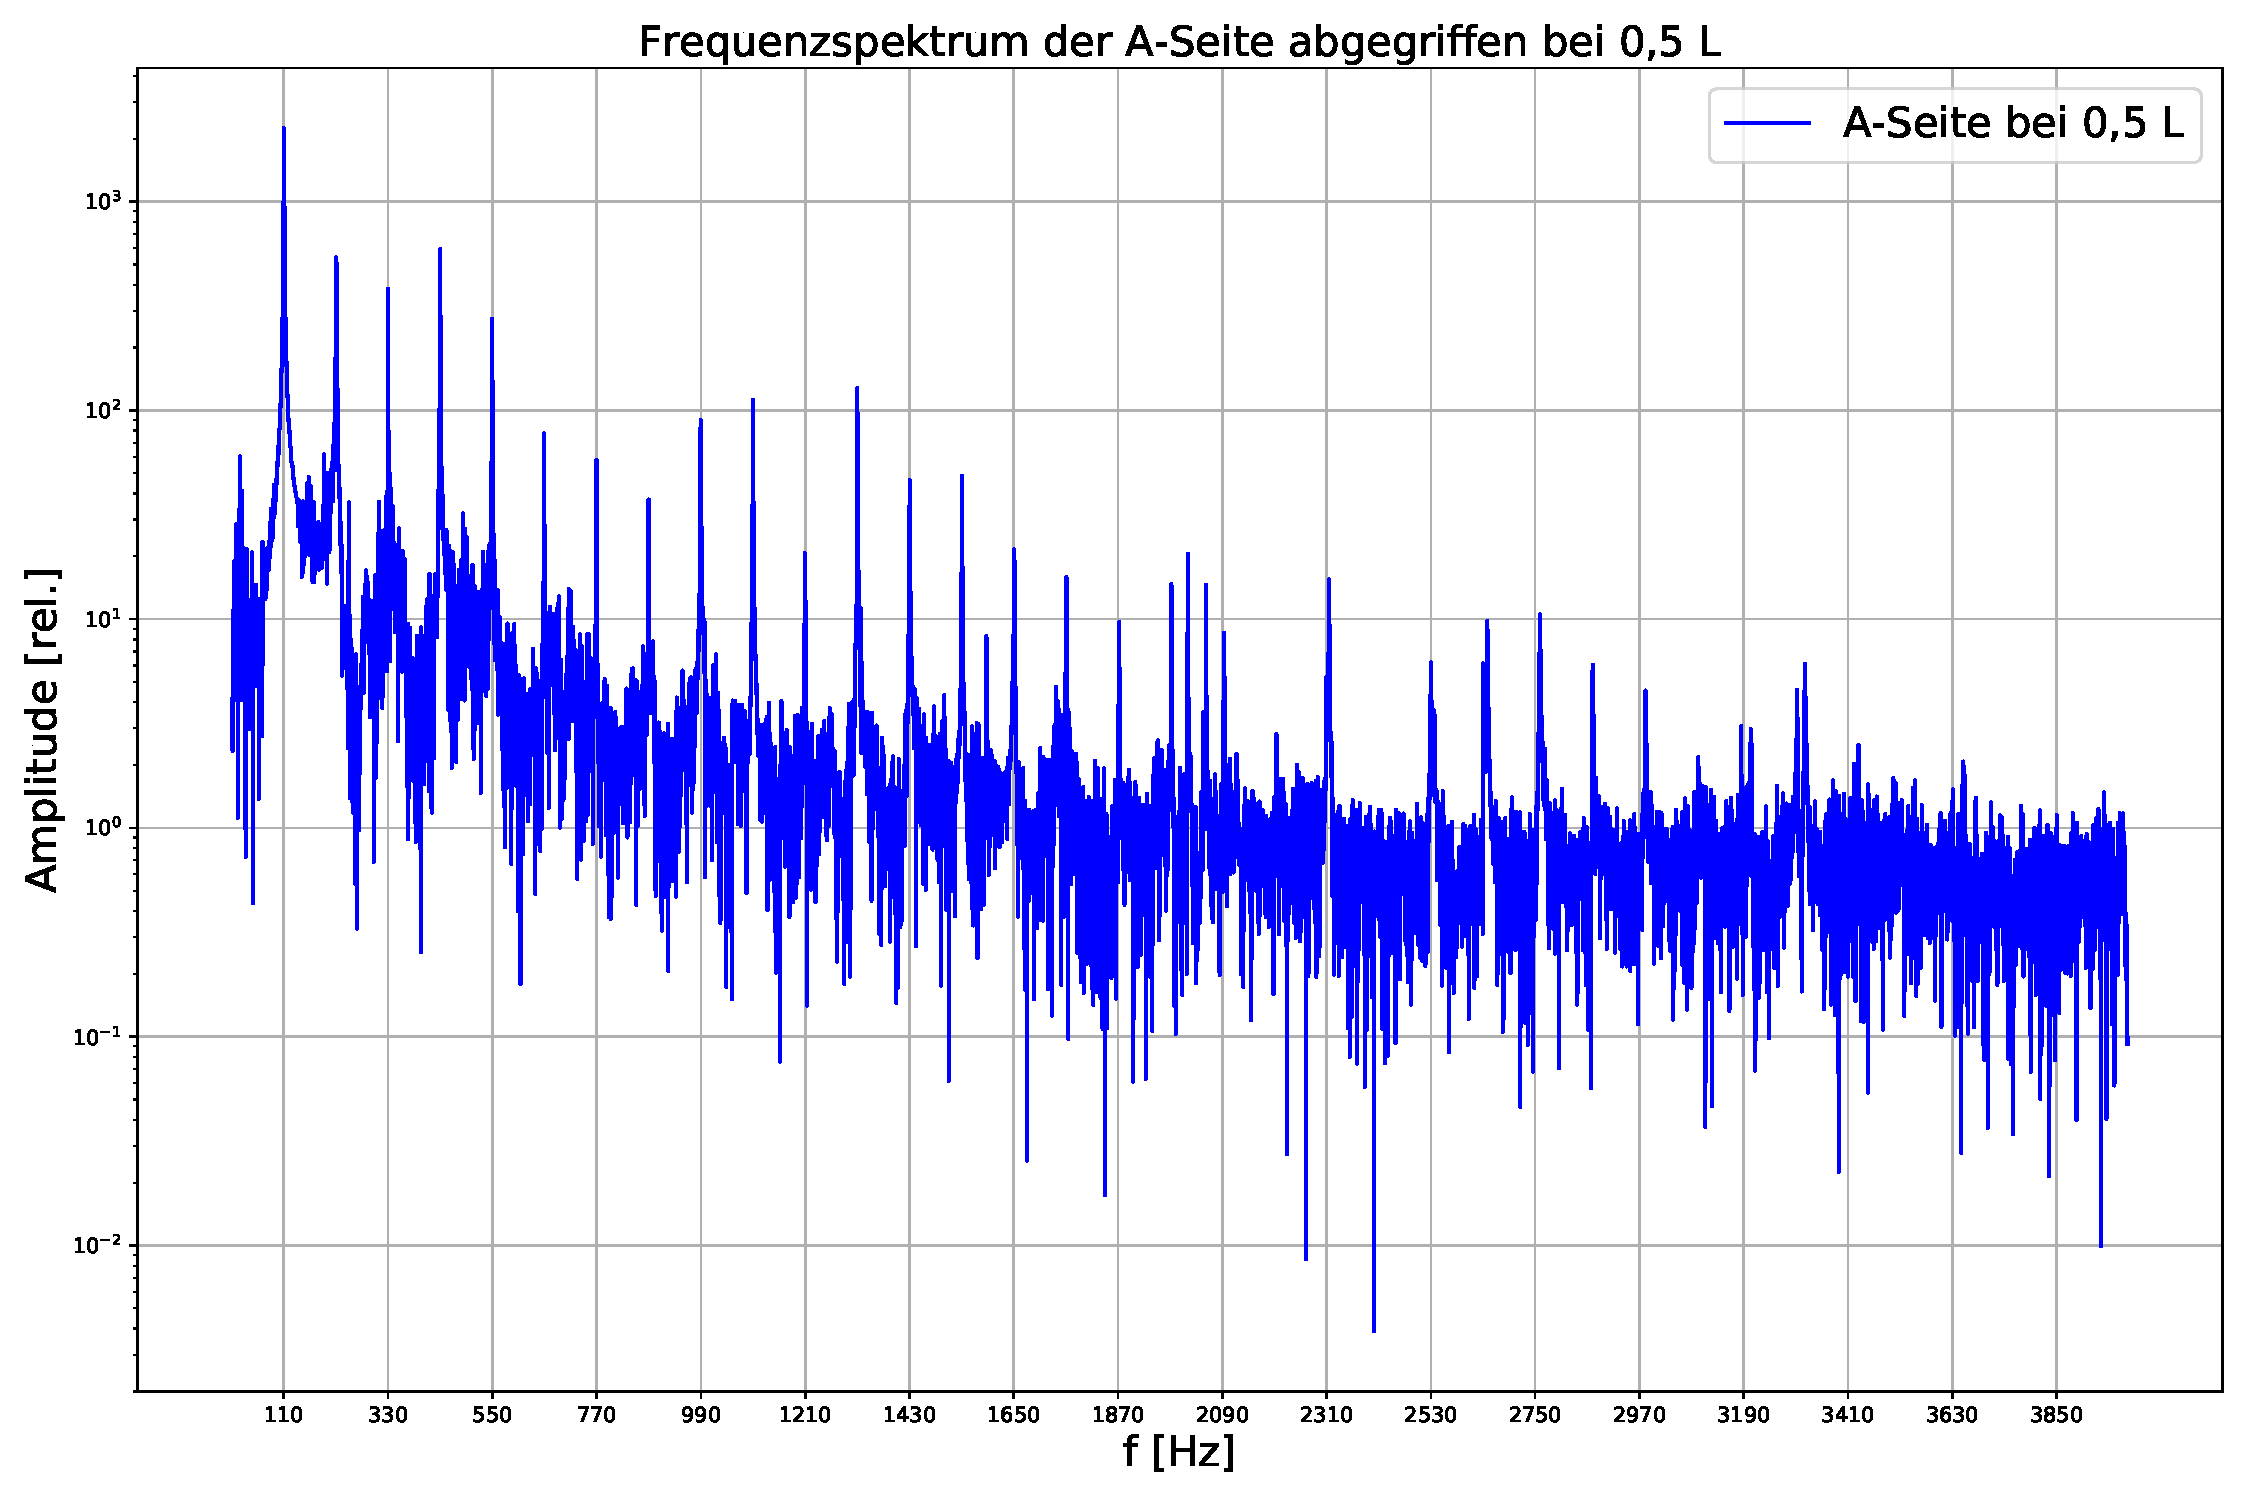
\includegraphics[scale=0.35]{../Plots/A-0,5.pdf}
	\caption{Frequenzspektrum der A-Saite, angeschlagen bei der Hälfte ihrer Länge}
	\label{fig:A-0,5}
\end{figure}

\begin{figure}[H]
	\centering
	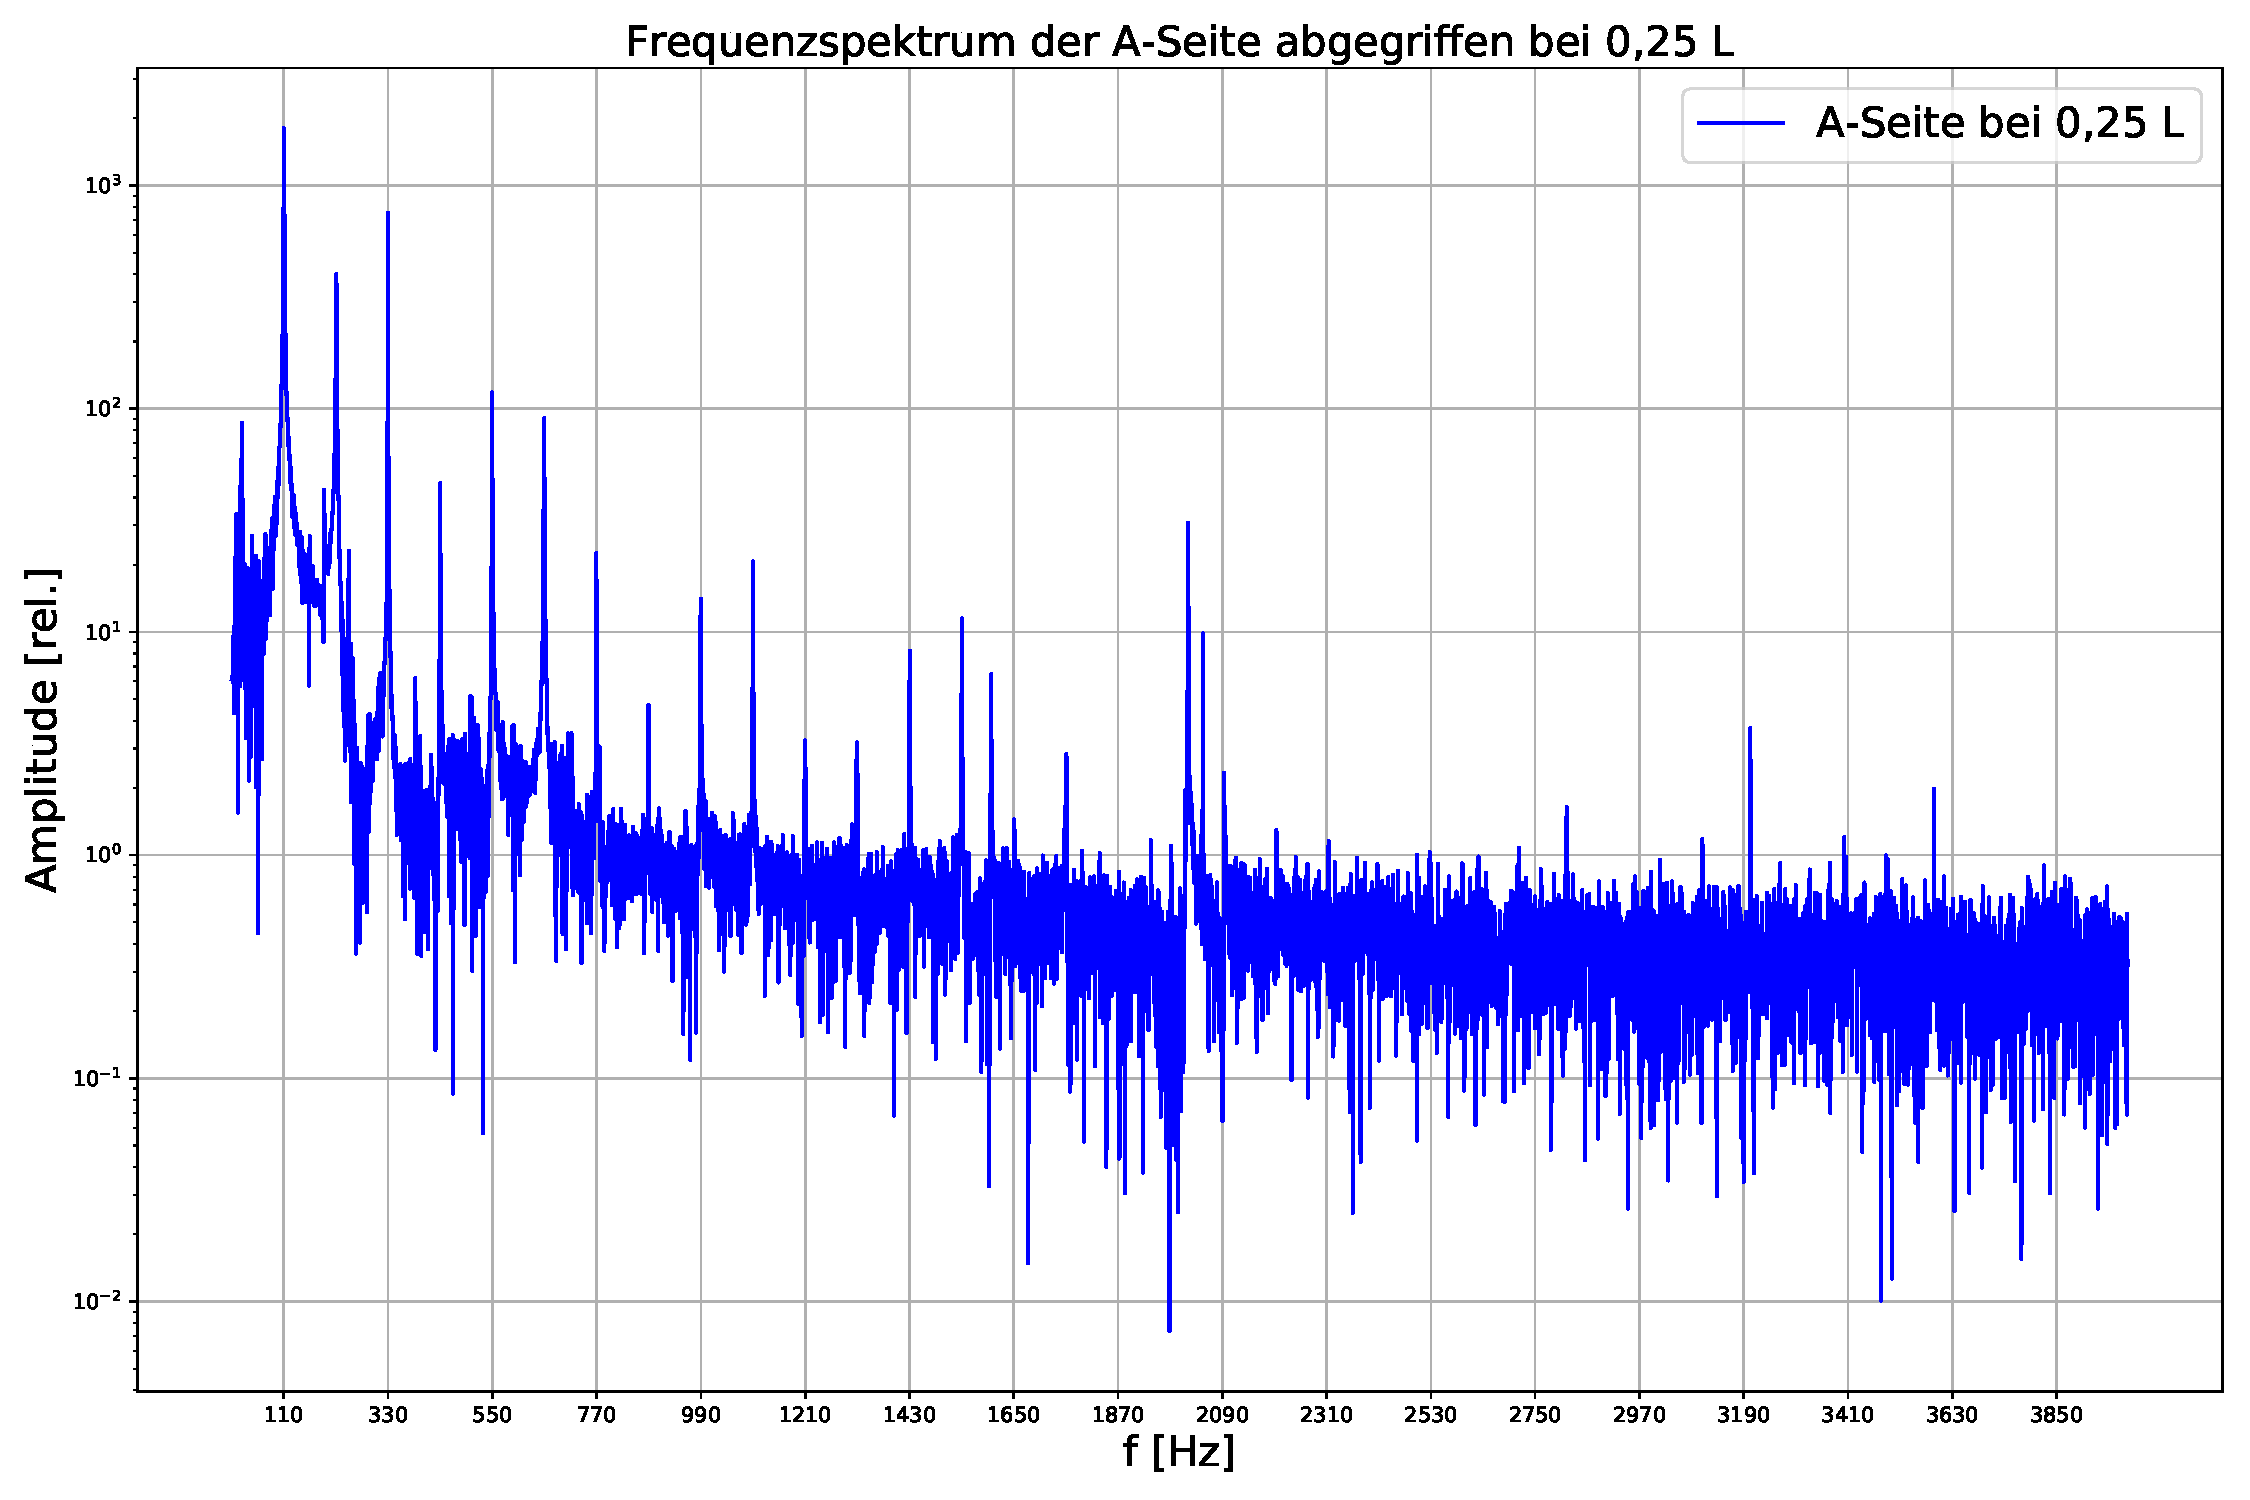
\includegraphics[scale=0.35]{../Plots/A-0,25.pdf}
	\caption{Frequenzspektrum der A-Saite, angeschlagen bei einem Viertel ihrer Länge}
	\label{fig:A-0,25}
\end{figure}

\subsection{Fazit}
Bei der Aufnahme der Schwebung musste zunächst die Saite in richtigem Maße verstimmt werden, da ansonsten keine Schwebung zustande kam. Die beiden bestimmten Schwebungsfrequenzen lagen nah beieinander, wobei der Fehler bei der Ablesemethode viel geringer ausfiel.

Die Bestimmung der Materialeigenschaften hat bei der A-Saite mit einer Abweichung von unter $3\,\sigma$ gut funktioniert, bei der E-Saite jedoch garnicht. Wir vermuten dass dies daran lag, dass diese Saite während des Versuchs versehentlich verstimmt wurde.

Bei der Aufnahme der Frequenzspektren bei verschiedenen Anschlägen der Saite konnte die Erwartung, dass ungerade Vielfache der Grundfrequenz nicht sichtbar werden, nicht bestätigt werden. Der logarithmische Abfall der Intensität der Oberschwingungen war jedoch relativ gut zu sehen.

\clearpage
\section{Anhang}
\begin{figure}[H]
	\centering
	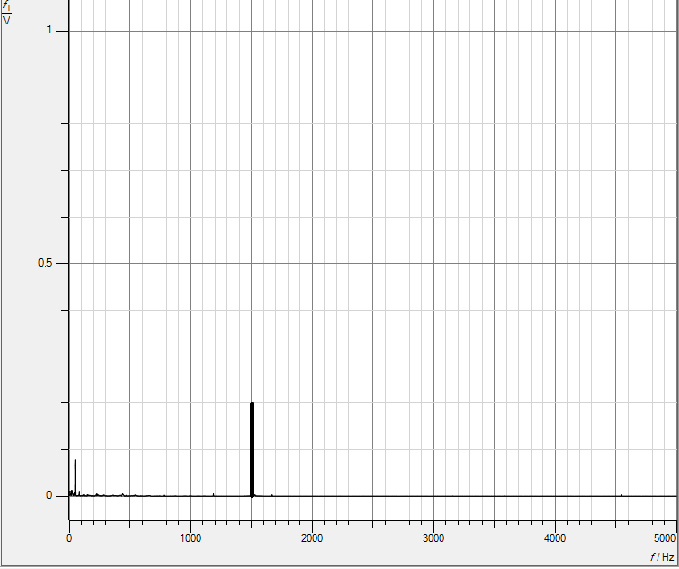
\includegraphics[scale=0.35]{../Kupfer.png}
	\caption{Frequenzspektrum einer Schwingung der Kupferstange}
	\label{fig:Kupfer}
\end{figure}
\begin{figure}[H]
	\centering
	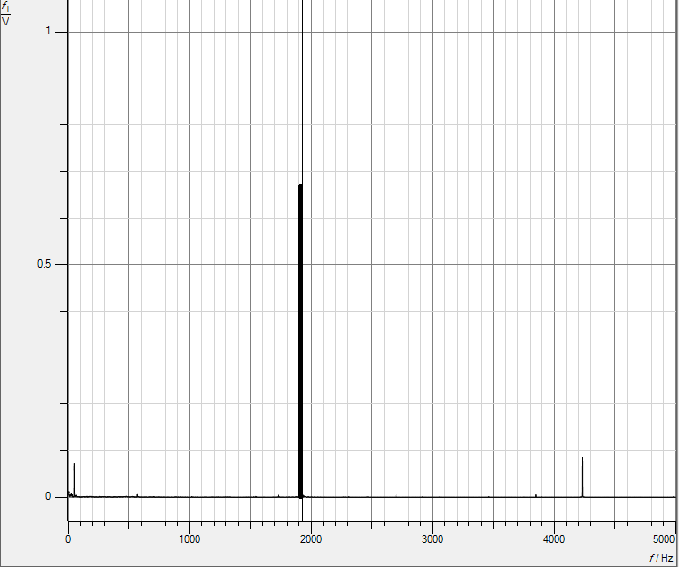
\includegraphics[scale=0.35]{../Messing.png}
	\caption{Frequenzspektrum einer Schwingung der Messingstange}
	\label{fig:Messing}
\end{figure}

\begin{figure}[H]
	\centering
	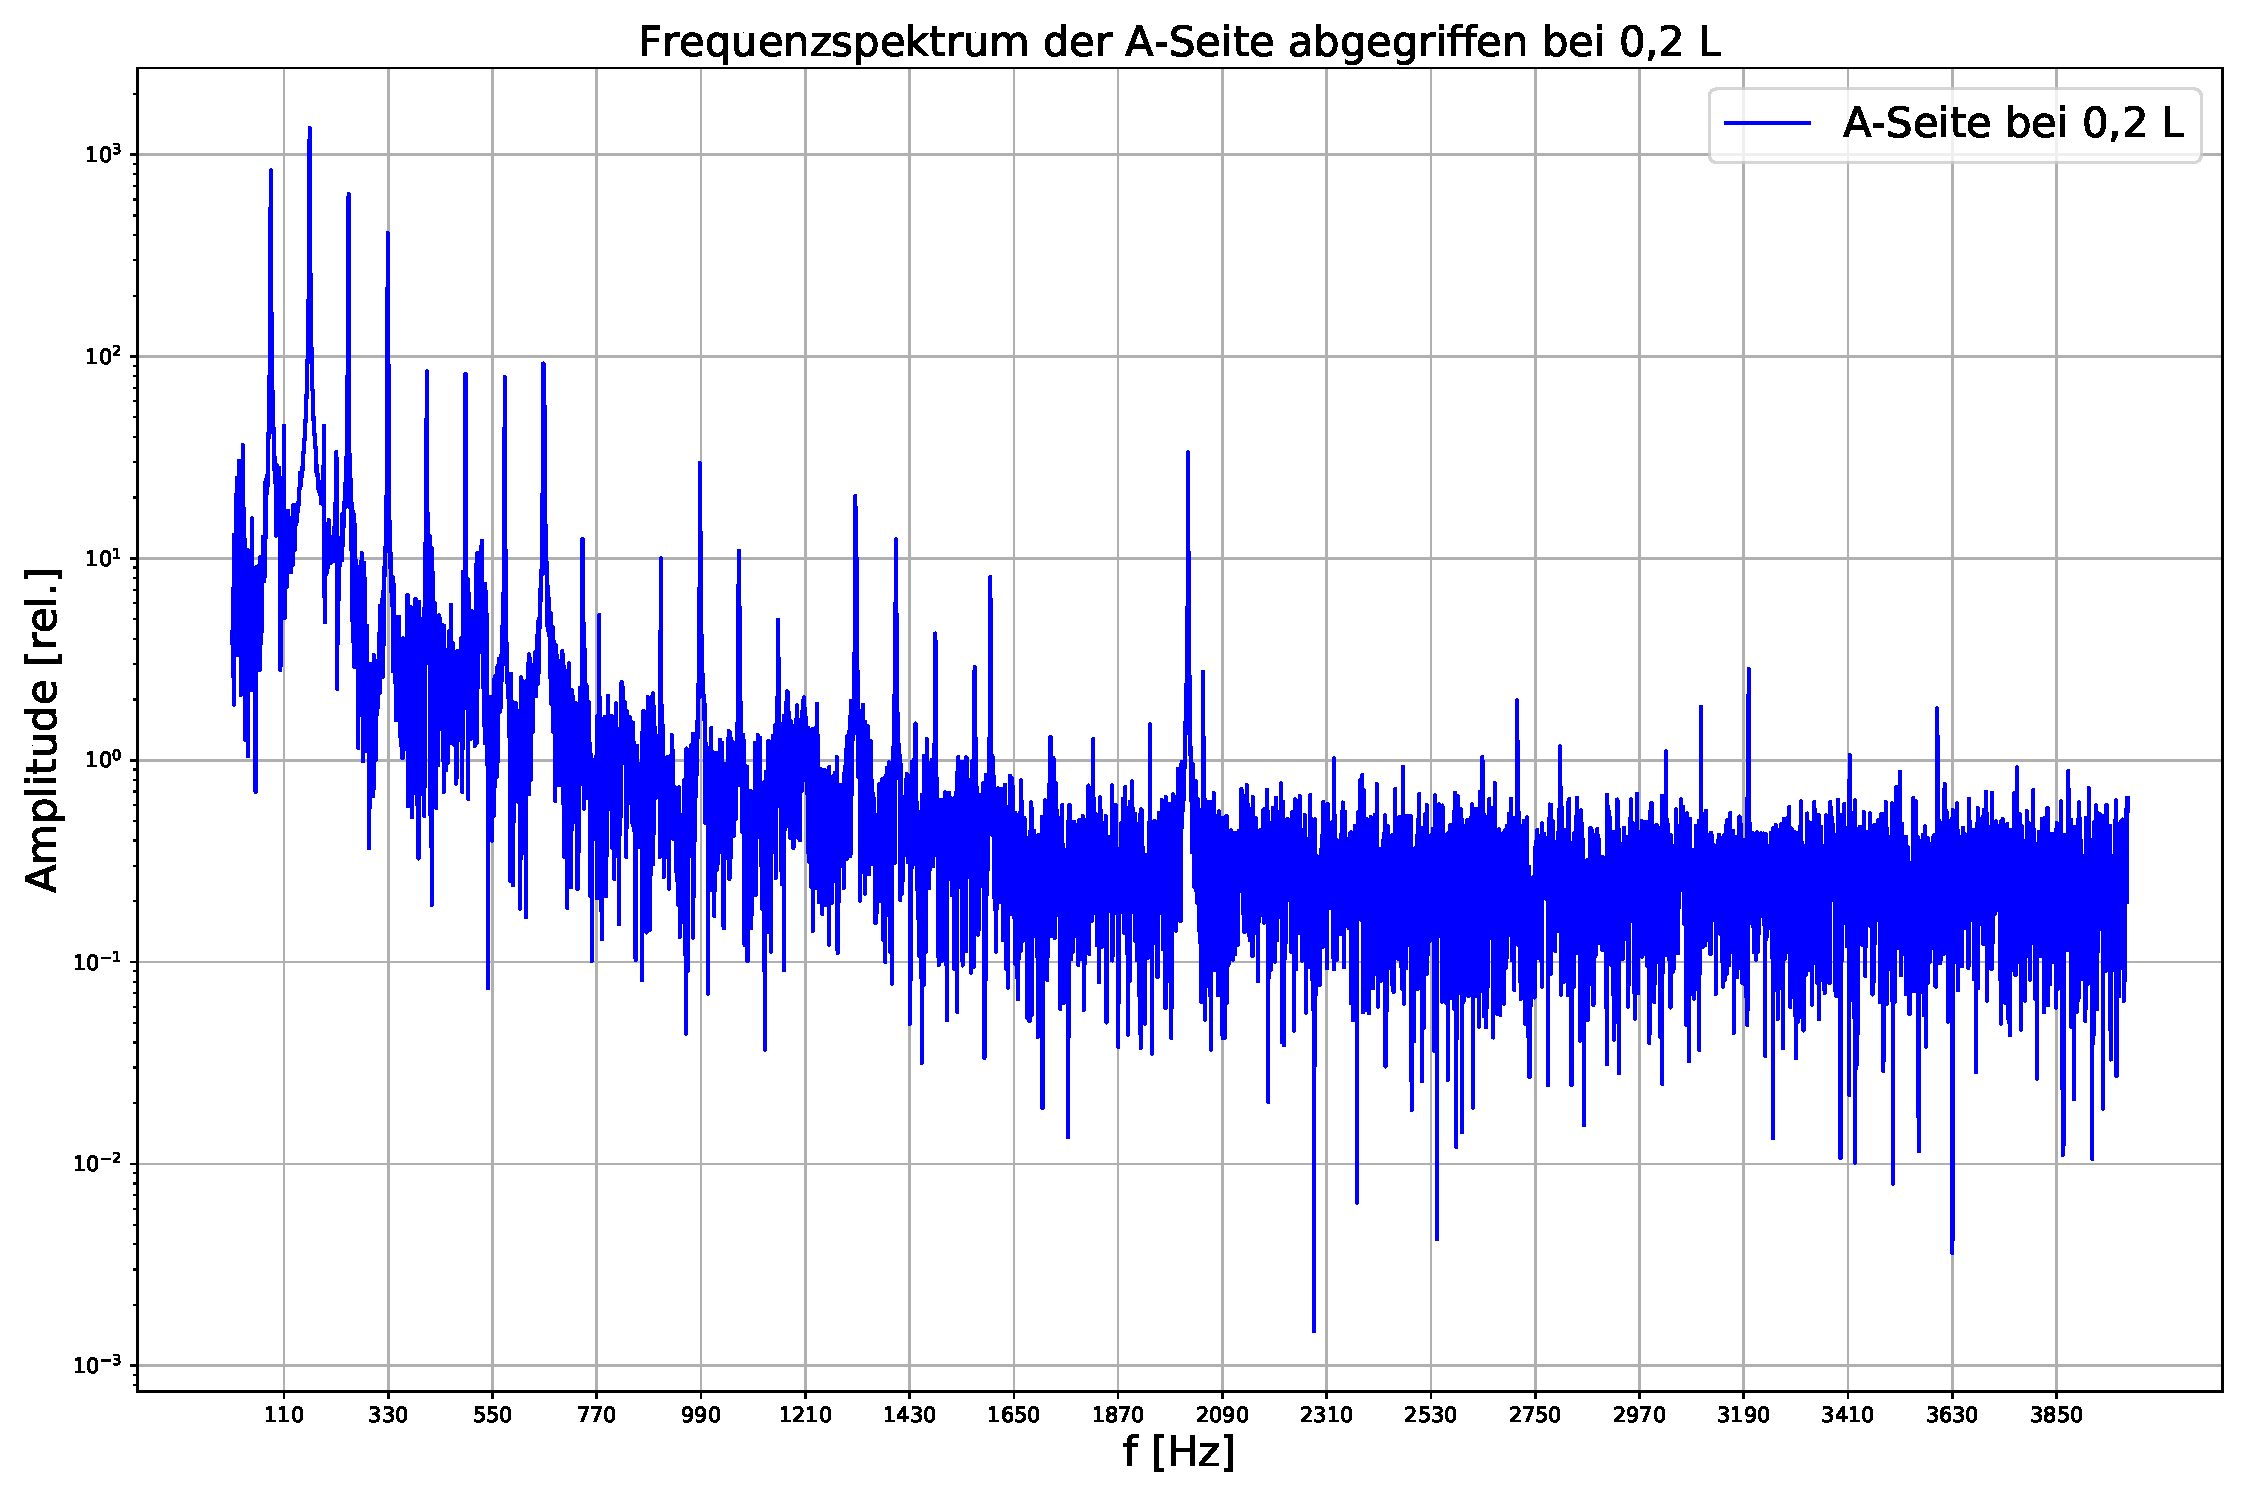
\includegraphics[scale=0.35]{../Plots/A-0,2.pdf}
	\caption{Frequenzspektrum der A-Saite, angeschlagen bei einem Fünftel ihrer Länge}
	\label{fig:A-0,2}
\end{figure}
\begin{figure}[H]
	\centering
	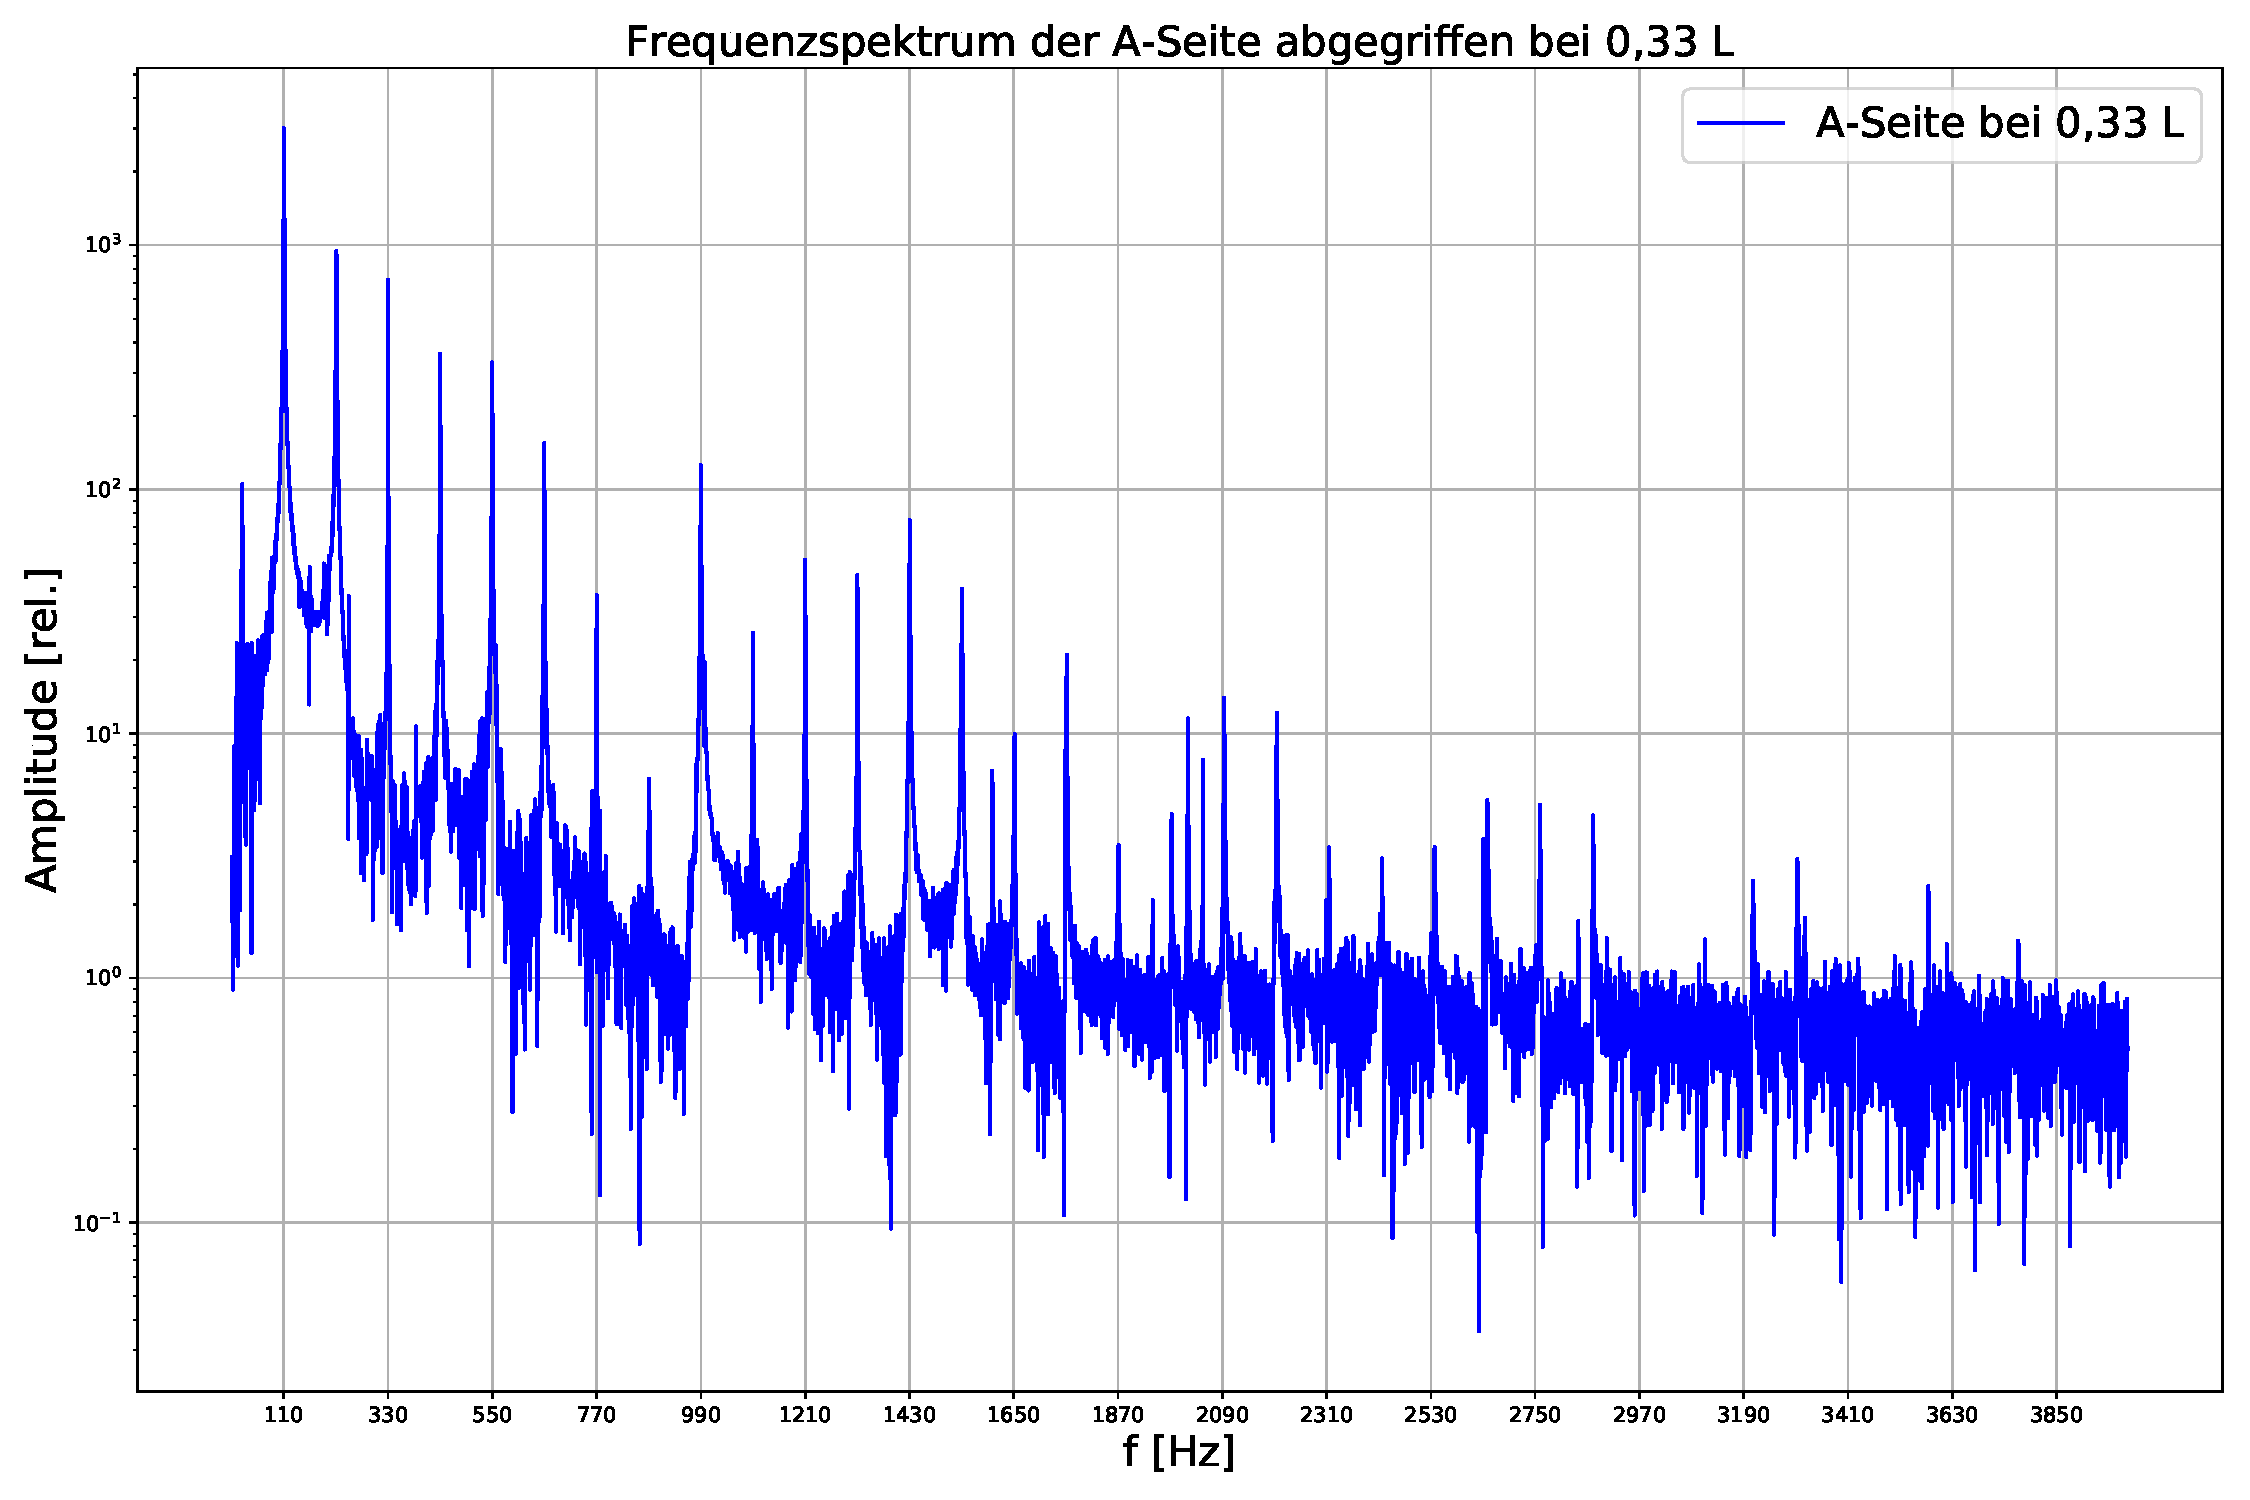
\includegraphics[scale=0.35]{../Plots/A-0,33.pdf}
	\caption{Frequenzspektrum der A-Saite, angeschlagen bei einem Drittel ihrer Länge}
	\label{fig:A-0,33}
\end{figure}
\begin{figure}[H]
	\centering
	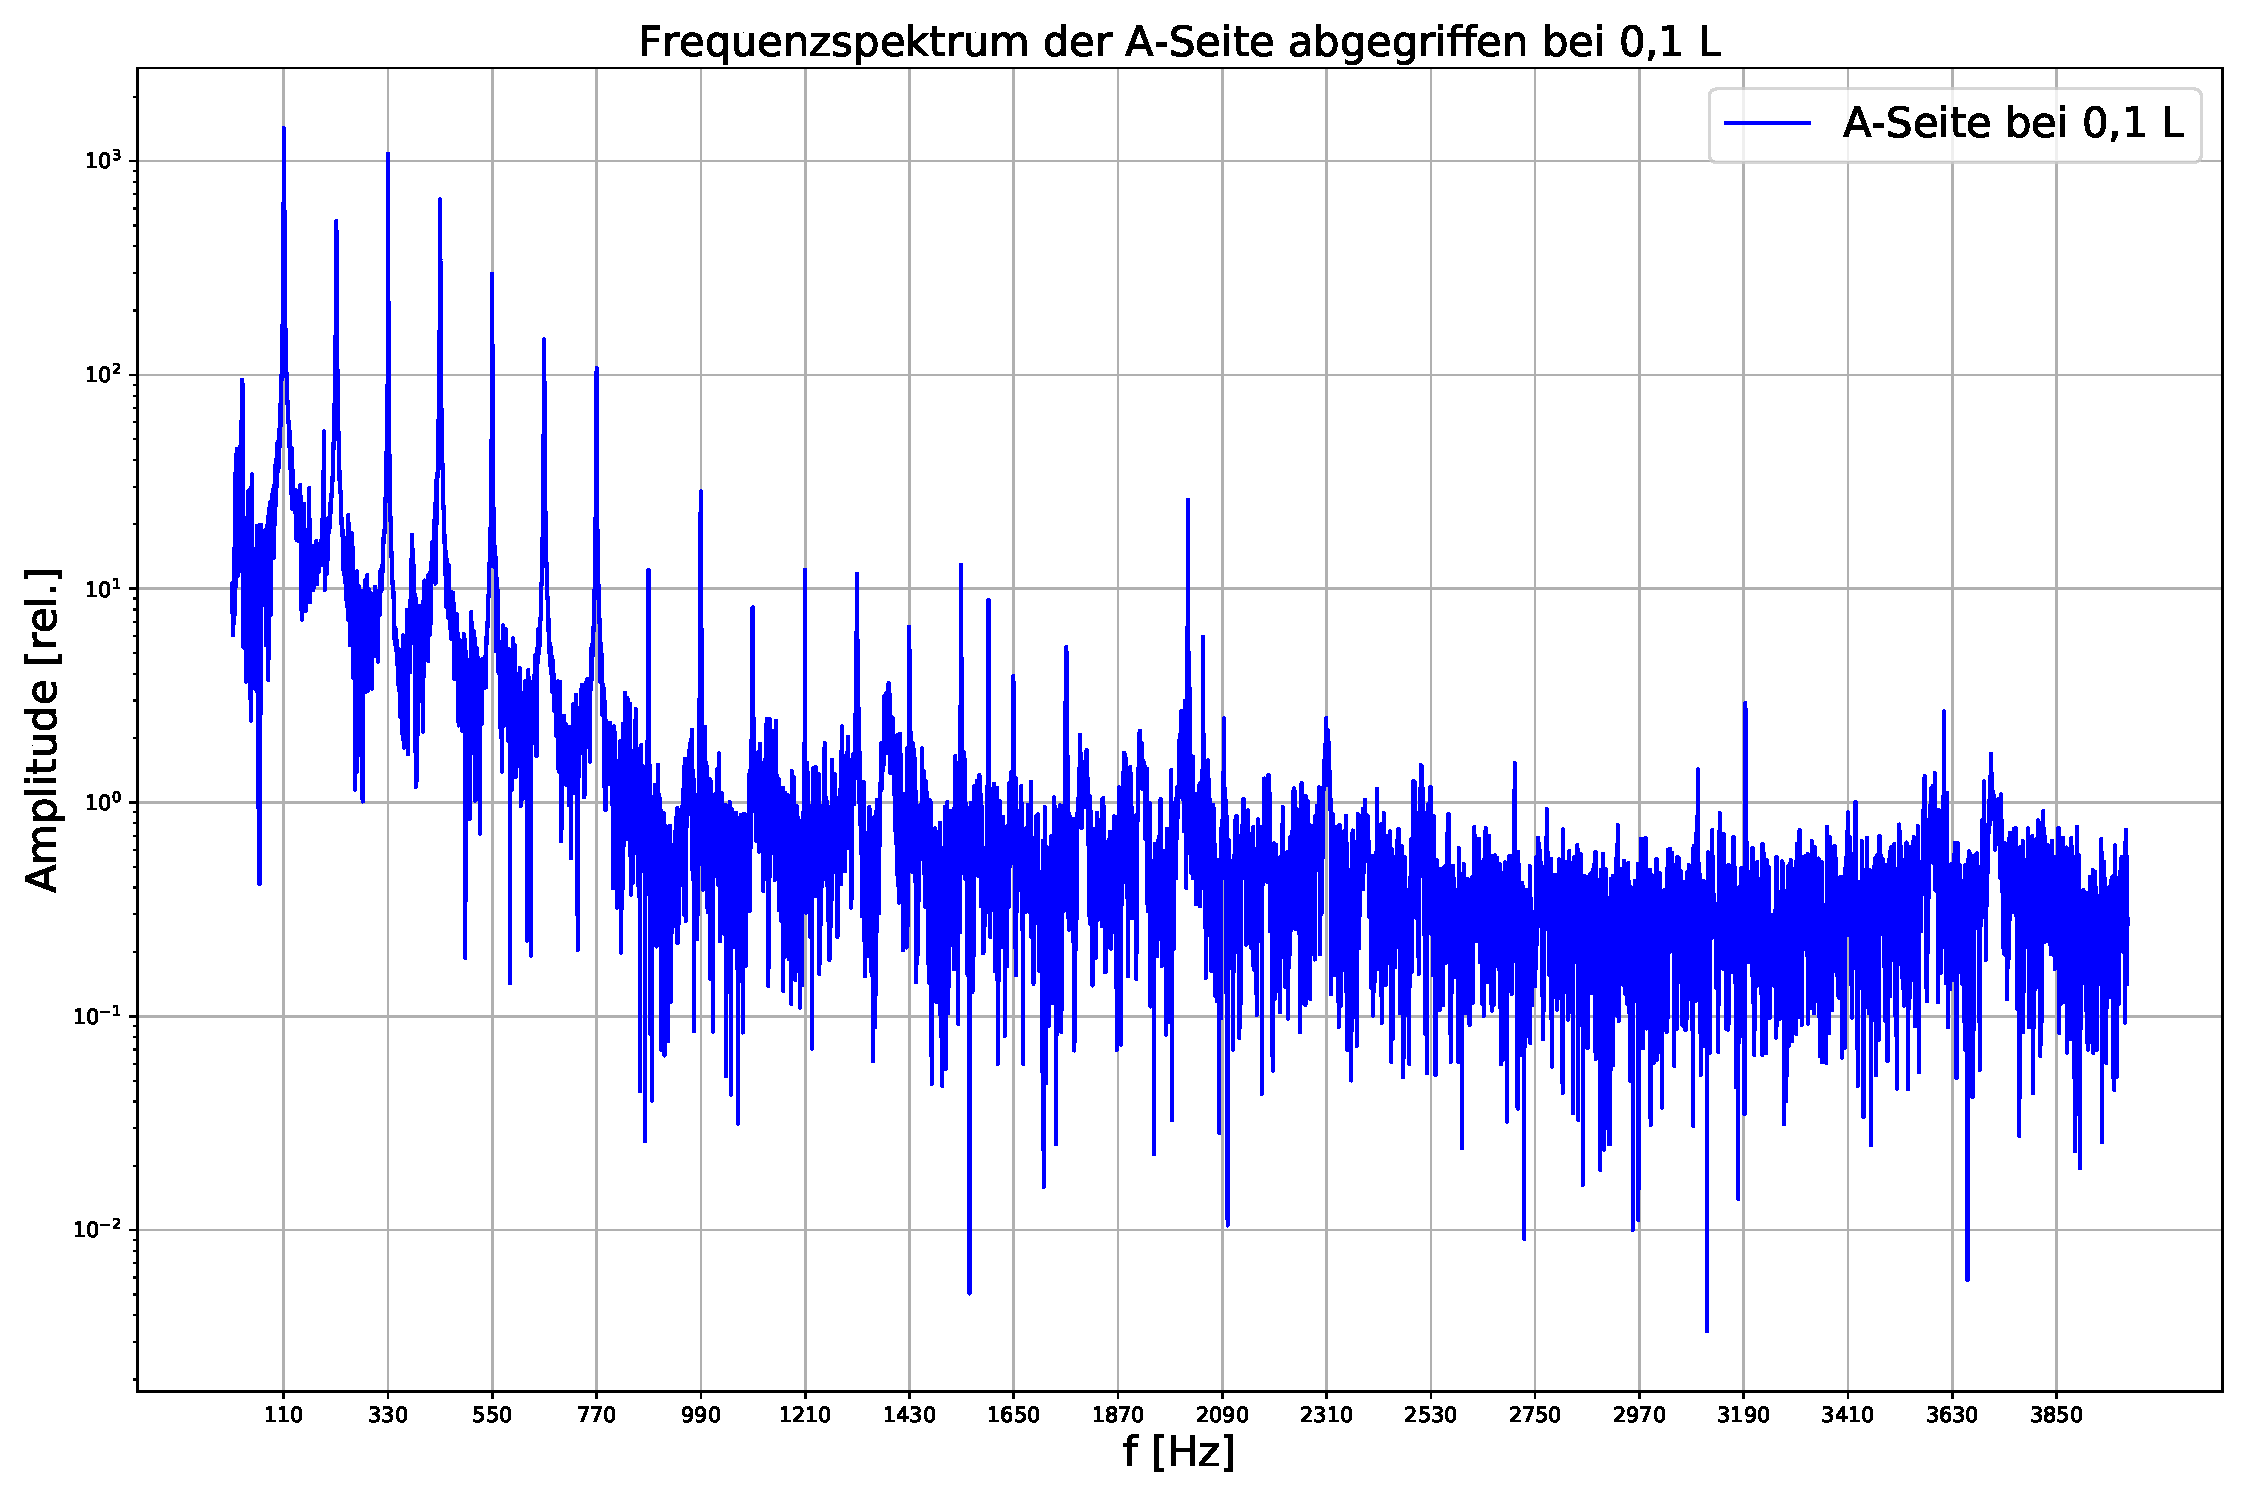
\includegraphics[scale=0.35]{../Plots/A-0,1.pdf}
	\caption{Frequenzspektrum der A-Saite, angeschlagen bei einem Zehntel ihrer Länge}
	\label{fig:A-0,1}
\end{figure}



\clearpage
\listoffigures
\listoftables

\end{document}

